\documentclass{article}
\usepackage{amsmath,amssymb}
\usepackage{graphicx,tikz,pgf}

\title{User's manual for \texttt{DISODE45}, a MATLAB integration code (v1.0)}
\author{M. Calvo$^{\mbox{\tiny {
1}}}$, Juan I. Montijano$^{\mbox{\tiny {
2}}}$ \& Luis R\'{a}ndez$^{\mbox{\tiny {
3}}}$}
%\affiliation[IUMA]{IUMA \\ Universidad de Zaragoza }
\date{\today}



\begin{document}

\maketitle

\begin{center}
{ \footnotesize\em Departamento  Matem\'{a}tica Aplicada\\
Pza. San Francisco s/n,
Universidad de Zaragoza.\\
50009-Zaragoza, Spain.}
\\[3pt]
 \footnotesize $^{\mbox{\tiny\rm 1}}$
email: calvo\symbol{'100}unizar.es
\\
 \footnotesize $^{\mbox{\tiny\rm 2}}$
 email: monti\symbol{'100}unizar.es
\\
 \footnotesize $^{\mbox{\tiny\rm 3}}$
email: randez\symbol{'100}unizar.es
\end{center}


\section{The DISODE45 function}
\texttt{DISODE45}  is a Matlab function that
solves non-smooth, non-stiff differential systems
\[
y'(t)=f(t,y(t)), \qquad  y(0)=y_0 \in \mathbb{R}^m, \qquad  t\in[t_0, t_f]
\]
The non-smoothness of the solution $y=y(t)$ happens at points, switching points, $(t_d, y_d)$ where  one
of several switching surfaces defined by a function $g(t,y)=(g_1(t,y), \ldots, g_k(t,y))$ vanish, that is,
at least for a index $i$, $g_i(t_d,y_d)=0$.

The call to this function has the following syntax

\begin{verbatim}
[T,Y] = disode45(odefun,switchfun,tspan,y0)
[T,Y,TDIS,YDIS,IDIS,STATS]=disode45(odefun,switchfun,tspan,y0)
[T,Y] = disode45(odefun,switchfun,tspan,y0,options)
[T,Y,TDIS,YDIS,IDIS,STATS]=disode45(odefun,switchfun,tspan,y0,options)
\end{verbatim}

It is very similar to the syntax used by the ODE suite Matlab package so that
users that are familiar with this software can find the use of
\texttt{disode45} very easy.

\medskip

\subsection{Input arguments}

\begin{description}
\item[odefun]
A function handle that evaluates the right side of the differential equations
$f(t,y)$.
\item[switchfun]
A function handle that evaluates the function $g(t,y)$ defining the switching
surfaces.
\item[tspan]
A vector specifying the interval of integration, $[t0,tf]$. The solver imposes the initial conditions at \texttt{tspan(1)},
and integrates from \texttt{tspan(1)} to \texttt{tspan(end)}.
For the moment, the code does not allow vectors \texttt{tspan} with more than two components, and $t_f$ must be greater than $t_0$
\item[y0]
A $m$ dimensional vector of initial conditions.
\item[options]
Structure of optional parameters that change the default integration properties.
You can create options using the disodeset function.
\end{description}

\subsection{Output arguments}

\begin{description}
\item[T]
Column vector of time points.
\item[Y]
Solution array. Each row in Y corresponds to the solution at a time returned in the corresponding row of T.
\item[TDIS]
Vector of times at which discontinuities or switching points of the numerical solution have been detected.
\item[YDIS]
The solution at the times of switching points. Each row in YDIS corresponds to the
solution at a time returned in the corresponding row of TDIS.
\item[IDIS]
Vector containing the indexes $i$ of the switching function that vanishes at each switching point.
\begin{itemize}
\item
The absolute value of \texttt{IDIS(i)} indicates the switching function corresponding to the $i$--eme switching point.
\item
The sign of \texttt{IDIS(i)} indicates the type
of discontinuity. It it is positive, the discontinuity is
transversal. If it is negative, the switching point is Filippov (entering or either exiting a sliding region).  For example, a value $\texttt{IDIS(4)}=-2$ means that the fourth switching point is a Filippov point located at the second switching surface $g_2(t,y)$.
\end{itemize}
\item[STATS]
Vector containing some statistics about the integration

\begin{tabular}{ll}
STATS(1) &  Number of accepted normal steps \\
STATS(2) &  Number of rejected normal steps \\
STATS(3) &  Number of accepted sliding steps\\
STATS(4) &  Number of rejected sliding steps\\
STATS(5) &  Number of steps at with a possible switching point\\
STATS(6) &  Number of transversal discontinuities \\
STATS(7) &  Number of sliding discontinuities \\
STATS(8) &  Number of exits of a sliding region\\
STATS(9) &  Number of calls to odefun\\
STATS(10) & Number of calls to switchfun \\
STATS(11) & Number of calls to gradswitchfun \\
\end{tabular}
\end{description}

\subsection{Required user's functions}
\begin{description}
\item[odefun]
The function,

\begin{verbatim}
f=odefun(t,y)
\end{verbatim}

\noindent for a scalar t and a column vector y, must return a column vector f corresponding to $f(t,y)$.
\item[switchfun]
The function

\begin{verbatim}
[value,isterminal,direction] = switchfun(t,y)
\end{verbatim}

\noindent for a scalar t and a column vector y, must return three column vectors
\begin{itemize}
\item
\texttt{value(i)}  is the value of the i-th component  $g_i(t,y)$
\item
\texttt{isterminal(i)} specifies the action to be taken when a zero of the function
$g_i(t,y)$ is found. It can take the values $-1$, $0$ or $1$.
\begin{itemize}
\item
\texttt{isterminal(i)}=1 means
that the integration must terminate at a zero of the $i$--th switching function.
\item
\texttt{isterminal(i)}=0 means that the integration must continue without any action.
\item
\texttt{isterminal(i)}=$-1$ means that the program must call an external function \texttt{actionatswitch(t,y)}, that should have been provided by the user in the options by means of disodeset function  (see sections \ref{disodeset}
and \ref{optionalfunctions}).
\end{itemize}
\item
\texttt{direction(i)} specifies which zeros of $g_i(t,y)$ have to be computed.
\begin{itemize}
\item
\texttt{direction(i) = 0} means  that all zeros are to be computed (the default).
\item
\texttt{direction(i) = +1} means that only the zeros where the switching function increases, that is,
it passes from negative to positive, must be computed.
\item
\texttt{direction(i) = -1}
means that only the zeros where the switching function decreases must be computed.
\end{itemize}
\end{itemize}
\end{description}

\subsection{Getting the code}
The code can be downloaded at http://iuma.unizar.es/en/research/software


\section{A simple first example}

Let us consider a simple mechanical system consisting on a mass $m=1$
atached to a fixed wall by a spring with stiffness coefficient 1, moving on a surface with a Coulomb friction
with friction coefficient $\mu$ so that the friction force is $F_C=\mu g =0.4$.

\medskip

\begin{center}
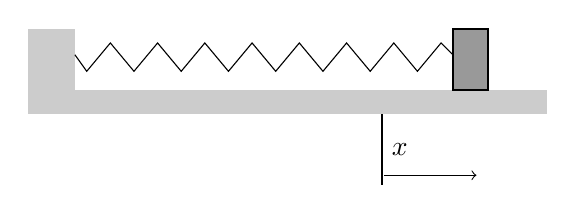
\begin{tikzpicture}[scale=3]
\draw (1.6,-0.2)-- (1.6,0.2);
\fill [black!20!white] (0.1,0.1) rectangle (2.3,0.2);
\fill [black!40!white] (1.9,0.20) rectangle (2.05,0.46);
\draw [thick] (1.9,0.20) rectangle (2.05,0.46);
\fill [black!20!white] (0.1,0.1)rectangle (0.3,0.46);
\draw (1.6,-0.05) node [right] {$x$};
\draw [->] (1.61,-0.16)-- (2.0,-0.16);
\draw (0.3,0.35) --(0.35,0.28) -- (0.45,0.40)-- (0.55,0.28) -- (0.65,0.40) -- (0.75,0.28) --
(0.85,0.40) --(0.95,0.28) -- (1.05,0.40) -- (1.15,0.28)-- (1.25,0.40) -- (1.35,0.28) --
(1.45,0.40) -- (1.55,0.28)-- (1.65,0.40) -- (1.75,0.28)-- (1.85,0.40) -- (1.9,0.35);
\end{tikzpicture}
\end{center}

\medskip

This system is modelled by the non-smooth second order differential equation
\[
x''  = - x - F_C \; \hbox{sign}(x').
\]

In order  to be
integrated by \texttt{DISODE45}, this second order equation must be expressed as a first order system with
two components $y_1(t)=x(t)$ and $y_2(t)=x'(t)$, as
\[
y'=\begin{pmatrix} y_1' \\y_2 '\end{pmatrix}=
\begin{pmatrix} y_2 \\ -y_1 - F_C \; \hbox{sign}(y_2)\end{pmatrix} = f(t,y)
\]

Clearly the vector field is non smooth at points where $x'=y_2=0$. Then, we have a
unique switching surface  $g(y_1,y_2)=y_2$.

The solution, with initial conditions $x(0) = 3,  x'(0)= 0$,
passes first through 3 transversal discontinuities and after that, at $t=12.5664\ldots$ it enters a sliding
region with  $x=0.2$, $x'=0$ and stays at this point forever (the friction force is greater
than the force of the spring and the mass stops).

The evolution of the solution $x(t)$ and its derivative $x'(t)$ are depicted in Figure \ref{Example0}.  The discontinuity points are indicated by means of small circles. Note that for this problem, since it is a second order differential equation,  the solution $x(t)$ and its derivative $x'(t)$
are continuous, as it can be seen in the plots, but the second derivative $x''(t)$ is not continuous.
\begin{figure}[h]
\begin{center}
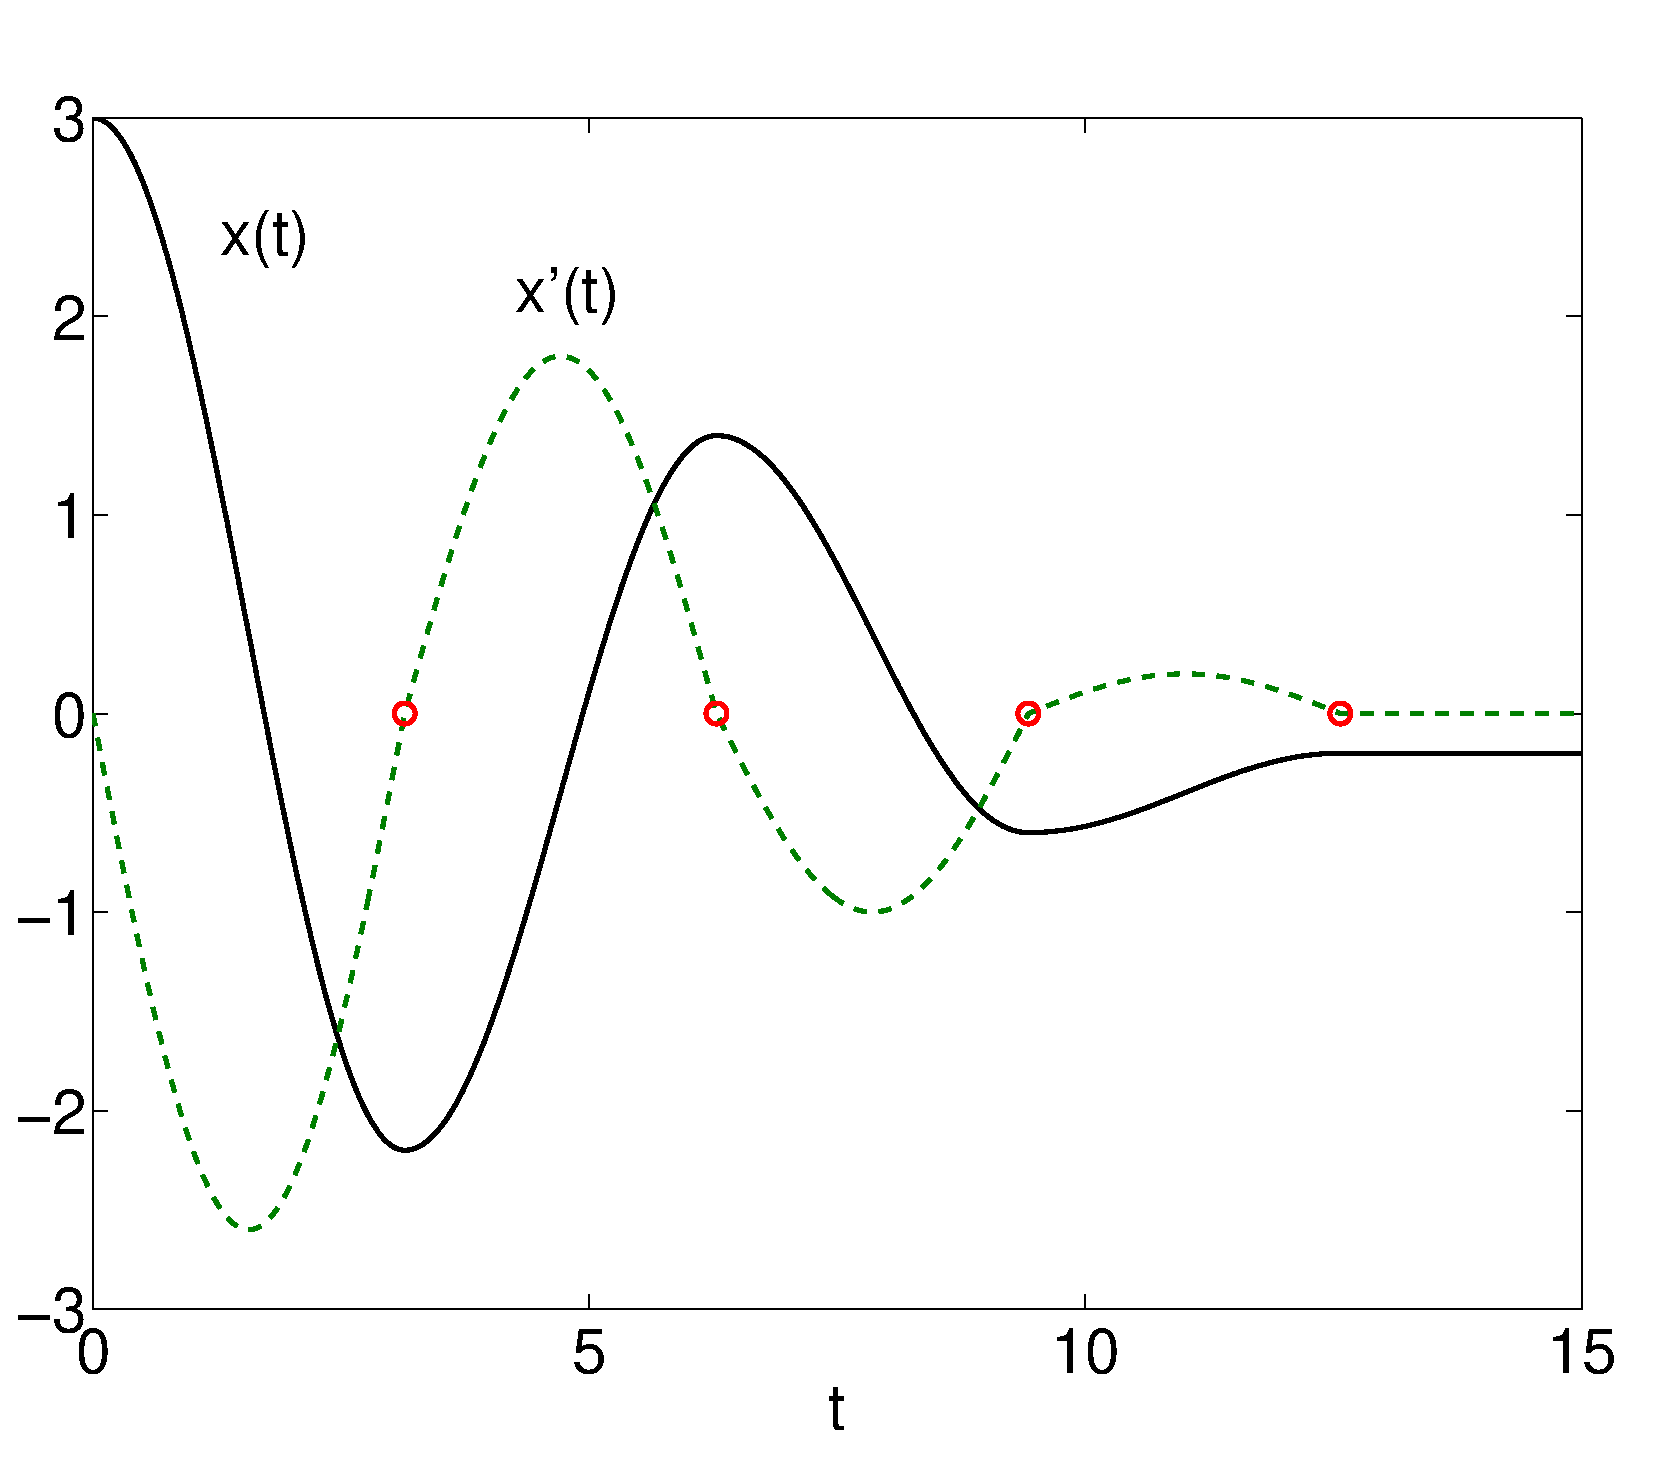
\includegraphics[width=6.2 true cm]{example0}
\quad
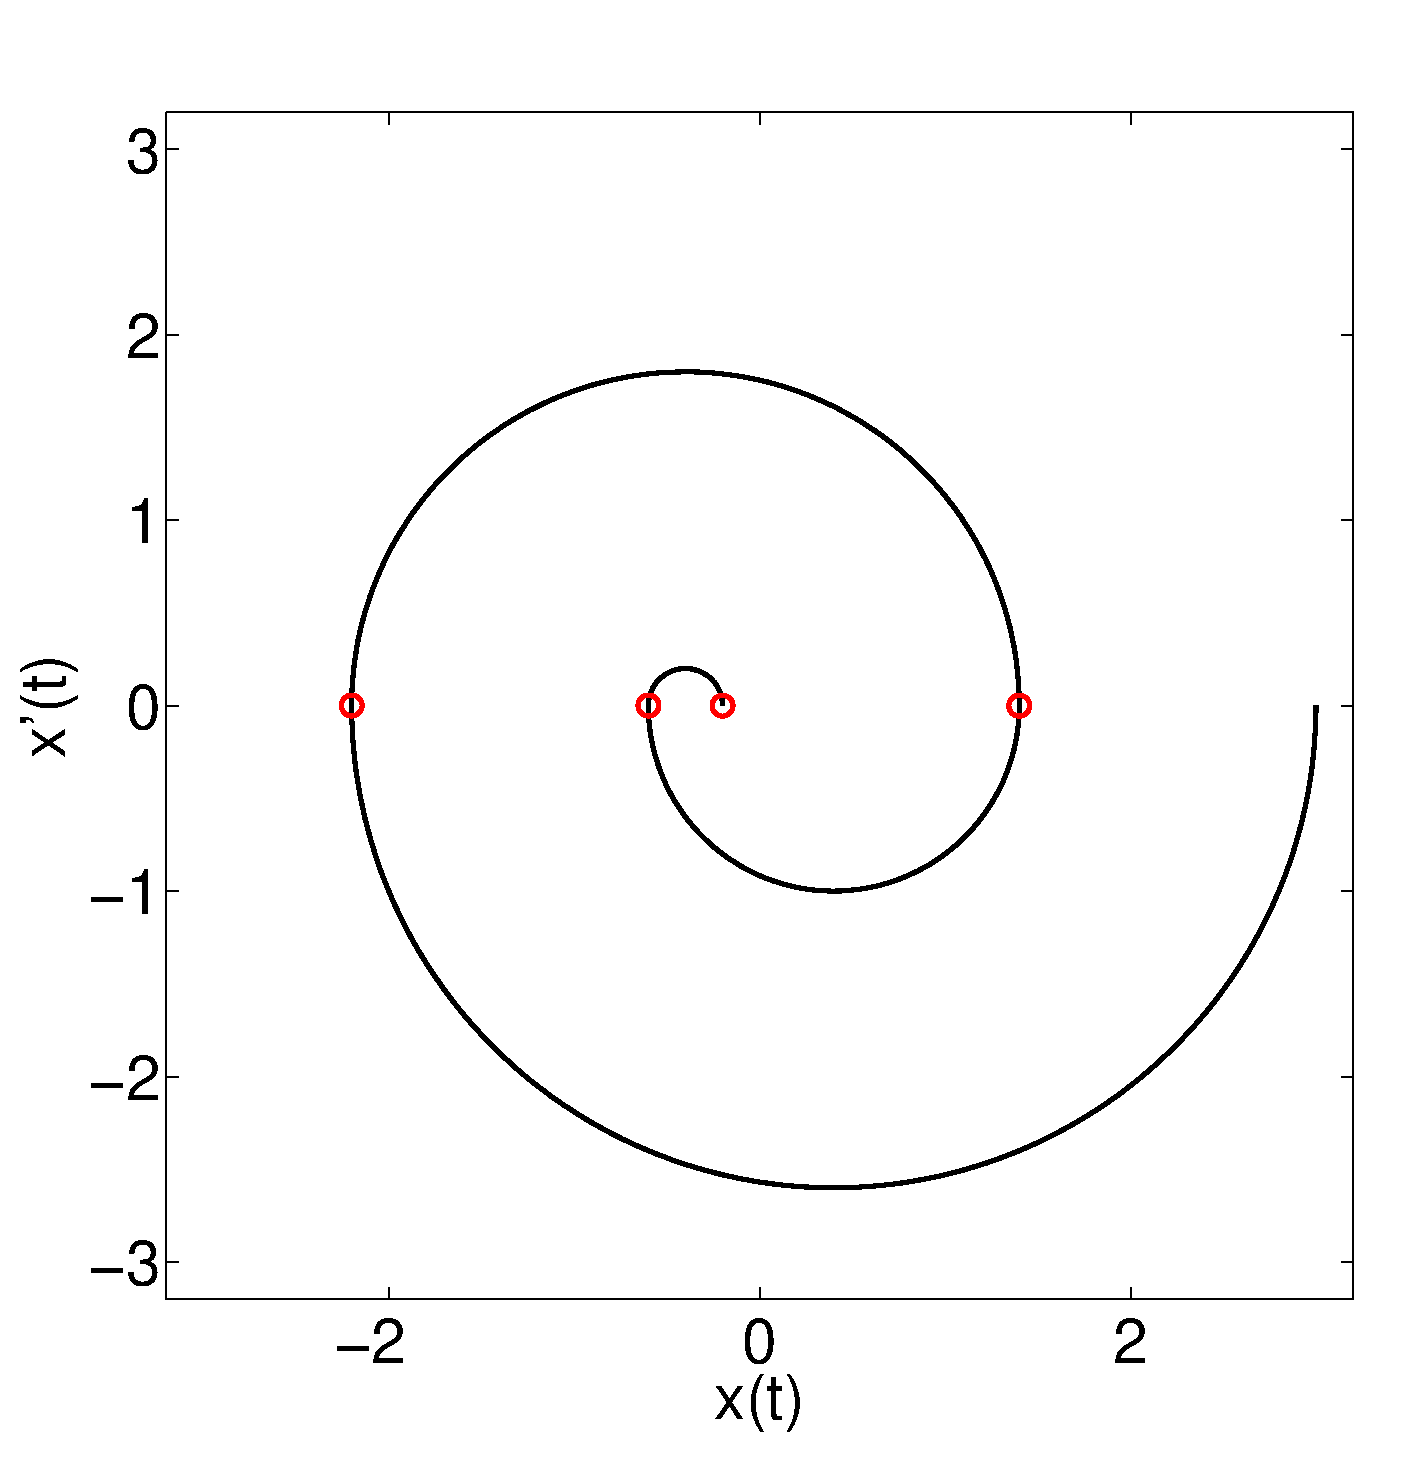
\includegraphics[width=5.4 true cm]{example0-phase}
\end{center}
\caption{Left:  Solution and derivative against time, Right:  Phase diagram}
\label{Example0}
\end{figure}

A Matlab code to integrate this problem with \texttt{disode45} can be

\bigskip

\begin{verbatim}
%
%  Call to disode45
%
 y0=[3;0];
 [tout,yout,tdis,ydis,idis,stats]=disode45(@fun, @gfun,[0,20], y0);
%
%  Definition of the vector field
%
 function f=fun(t,y)
      Fc=0.4;
      f=[y(2);-y(1)-Fc*sign(y(2))] ;
 end
%
%  Definition of the switching surface
%
 function [g,isterminal,direction]=gfun(t,y)
      g=y(2);
      isterminal=0;
      direction=0;
 end
\end{verbatim}

Once the integration of this problem has concluded, the vectors \texttt{tdis},
\texttt{ydis} and \texttt{idis}
contain the following data

\begin{verbatim}
tdis =

     0    3.1416    6.2831    9.4247   12.5661

ydis =

    3.0000         0
   -2.2000   -0.0000
    1.3999   -0.0000
   -0.5999    0.0000
   -0.2001   -0.0000

idis =

     1     1     1     1    -1
\end{verbatim}

The elements of the vector \texttt{idis} indicate that all the switching points correspond to the first
switching surface, an expected fact because there is a unique switching surface.
The first four components are positive, which means that these discontinuities are transversal.
The last one is negative, and therefore this discontinuity starts a sliding region.
Note that the integration starts at an initial condition $(3, 0)$ which belongs to the switching surface.
This is why the vector \texttt{tdis} has $0$ as its first element, which means that there is a switching point at $t=0$.

The plots shown in Figure \ref{Example0} (without legends) can be obtained with the matlab orders

\begin{verbatim}
plot(tout,yout(:,1),'k',tout,yout(:,2),'k--',tdis,ydis(:,2),'ro')

plot(yout(:,1),yout(:,2),'k-',ydis(:,1),ydis(:,2),'ro')
\end{verbatim}


\section{The DISODESET function}
\label{disodeset}
\texttt{DISODESET}  is a Matlab function that creates a options structure
that lets the user
set some parameters (options) to be used by \texttt{DISODE45}
in the numerical integration.

The call to this function has the following syntax

\begin{verbatim}
options=disodeset('name1',value1,'name2',value2,...)
\end{verbatim}

\medskip

\subsection{Allowed options}
\begin{description}
\item['RelTol']
Sets the Relative error tolerance  (default to  1e-3).
Each integration step satisfies $||est||_2 \le RelTol*||y||_2+AbsTol$.
\item['AbsTol']
Sets the absolute error tolerance  (default to  1e-6).
 See RelTol.
\item['InitialStep']
Sets a suggested initial step size and must be a positive scalar.
      The solver will try this first.  By default the solver determine an
      initial step size automatically.
\item['EventControl']
Sets the type of control for the detection of discontinuities
\begin{itemize}
\item[0]   Existence of discontinuity is checked at every step and every
          stage of failed steps.
\item[1]   Existence of discontinuity is checked at every stage of every
          step.
\item[k]   Existence of discontinuity is checked at every stage of every
          step and at 6*k uniformly distributed points inside every step.
\end{itemize}
\item['Refine']
Sets the output refinement factor and must be a positive integer.
This property increases the number of output points by the specified
      factor producing smoother output. Refine defaults to 4.
\item['Gradient']
Specifies, by means of a function handle, the function to compute the
gradient of the switching functions.
\item['ActionSwitch']
Specifies, by means of a function handle, the function to be called
by the integrator when a switching point is found.
This output function is called if the corresponding value of the vector \texttt{isterminal} is $-1$. ActionSwitch defaults to [\ ].
\end{description}

\section{Optional functions that can be provided by the user}
\label{optionalfunctions}

\begin{description}
\item[gradswitchfun]
The function

\begin{verbatim}
grad = gradswitchfun(t,y,inddis)
\end{verbatim}

\noindent for a scalar \texttt{t}, column vector \texttt{y}, and a switching function index \texttt{inddis}, must return a column vector grad which is the gradient vector
of the function $g_{\scriptsize\hbox{inddis}}$

This function must be provided by the user if the option 'Gradient' is set.  By default,
disode45 computes the gradient vector by means of divided differences.

\item[actionatswitch]
The function

\begin{verbatim}
yout = actionatswitch(t,y)
\end{verbatim}

\noindent for a scalar \texttt{t} and a column vector \texttt{y}, must return a column vector \texttt{yout} which is the new state vector.  The integration will proceed from the point
$t$ with the initial condition \texttt{yout}.

This function must be provided if the option 'ActionSwitch' is set, and it is executed if the function \texttt{switchfun(t,y)} returns a value -1 in the vector
\texttt{isterminal} at the switching point.
\end{description}

\section{Examples}
\begin{description}
\item[Example 1]
In the first example
we consider two masses $m_1=m_2=1$ linked by a spring, moving on a surface with Coulomb friction (see \cite[pp. 162]{AcaBro:08}).
Both masses are equal, but made with different material, so their friction coefficients $\mu_1$ and $\mu_2$
are different and so are the friction forces $F_1$ and $F_2$. The surface where the masses move has two
physically different parts, which makes the friction coefficients change.

\begin{center}
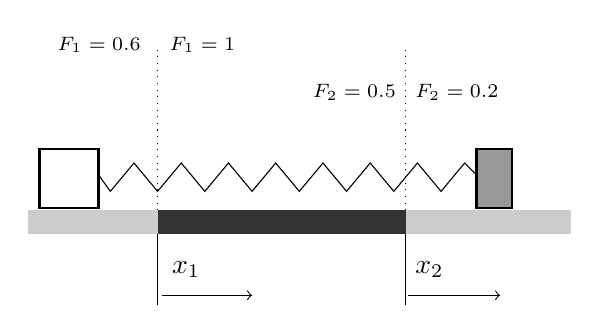
\begin{tikzpicture}[scale=3]
\draw (0.55,-0.2)-- (0.55,0.2);
\draw (1.6,-0.2)-- (1.6,0.2);
\draw [dotted] (0.55,0.2)-- (0.55,0.9);
\draw (0.52,0.9) node [left] {\scriptsize $F_{1}=0.6$};
\draw (0.56,0.9) node [right] {\scriptsize $F_{1}=1$};
\draw [dotted] (1.6,0.2)-- (1.6,0.9);
\draw (1.6,0.7) node [left] {\scriptsize $F_{2}=0.5$};
\draw (1.6,0.7) node [right] {\scriptsize $F_{2}=0.2$};
\fill [black!80!white] (0.54,0.1)rectangle (1.6,0.2);
\fill [black!20!white] (0.0,0.1)rectangle (0.55,0.2);
\fill [black!20!white] (1.6,0.1)rectangle (2.3,0.2);
\fill [black!40!white] (1.9,0.21) rectangle (2.05,0.46);
\draw [thick] (1.9,0.21) rectangle (2.05,0.46);
\draw [thick] (0.05,0.21)rectangle (0.3,0.46);
\draw (0.57,-0.05) node [right] {$x_{1}$};
\draw [->] (0.57,-0.16)-- (0.95,-0.16);
\draw (1.6,-0.05) node [right] {$x_{2}$};
\draw [->] (1.61,-0.16)-- (2.0,-0.16);
\draw (0.3,0.35) --(0.35,0.28) -- (0.45,0.40)-- (0.55,0.28) -- (0.65,0.40) -- (0.75,0.28) --
(0.85,0.40) --(0.95,0.28) -- (1.05,0.40) -- (1.15,0.28)-- (1.25,0.40) -- (1.35,0.28) --
(1.45,0.40) -- (1.55,0.28)-- (1.65,0.40) -- (1.75,0.28)-- (1.85,0.40) -- (1.9,0.35);
\end{tikzpicture}
\end{center}

This mechanical system is modelled by the non-smooth differential system


\[
\begin{cases}
x_1''  = - (x_1 - x_2) - F_1 \hbox{sign}(x_1'),  & \\
x_2''  = - (x_2 - x_1) - F_2 \hbox{sign}(x_2'),  & \\[4pt]
F_1=
\begin{cases}
1 & \hbox{ if } x_1 \le 0 \\
0.6  &\hbox{ if } x_1 > 0
\end{cases}
\qquad \quad
F_2=
\begin{cases}
0.5 & \hbox{ if } x_2 \le 0 \\ 0.2 & \hbox{ if } x_2 > 0
\end{cases}
\\
x_1(0) = -2, \ x_2(0)=3, \ x_1'(0)= 0, \ x_2'(0)=0  \vrule width 0pt height 16pt \\
t\in[0,6].
\end{cases}
\]
Again, we must express the second order system as a first order system with
four components $y_1(t)=x_1(t)$, $y_2(t)=x_2(t)$, $y_3(t)=x_1'(t)$ and $y_4(t)=x_2'(t)$)
\[
y'=\begin{pmatrix} y_1' \\y'_2 \\y'_3 \\y'_4\end{pmatrix}=
\begin{pmatrix} y_3 \\ y_4 \\ - (y_1 - y_2) - F_1\; \hbox{sign}(y_3) \\
- (y_2 - y_1) - F_2\; \hbox{sign}(y_4)
\end{pmatrix} = f(t,y)
\]

Clearly the vector field $f(t,y)$ is non smooth at points where $x'_1=y_3=0$, $x'_2=y_4=0$,
$x_1=y_1=0$ or $x_2=y_2=0$. Then, we have four switching surfaces  $g_1(y)=y_1$, $g_2(y)=y_2$,
$g_3(y)=y_3$ and $g_4(y)=y_4$.

The solution, with these initial conditions,
passes first through 14 transversal discontinuities and after some time it enters a sliding
region onto $g_1(y)=0$.  Inside this sliding region, $y_1=0$, the solution crosses three times transversal
discontinuities and finally
it attains a co-dimension 2 sliding region $y_3=y_4=0$, where both masses do not move, and
the system remains there forever.  The integrator stops when it find a co-dimension 2 Filippov point.

The components of the solution $x_1(t)$ and $x_2(t)$ of this problem as well as their derivatives are depicted in Figure \ref{Example1}.  The 18 discontinuity points are indicated by means of small circles.
\begin{figure}[!h]
\centerline{
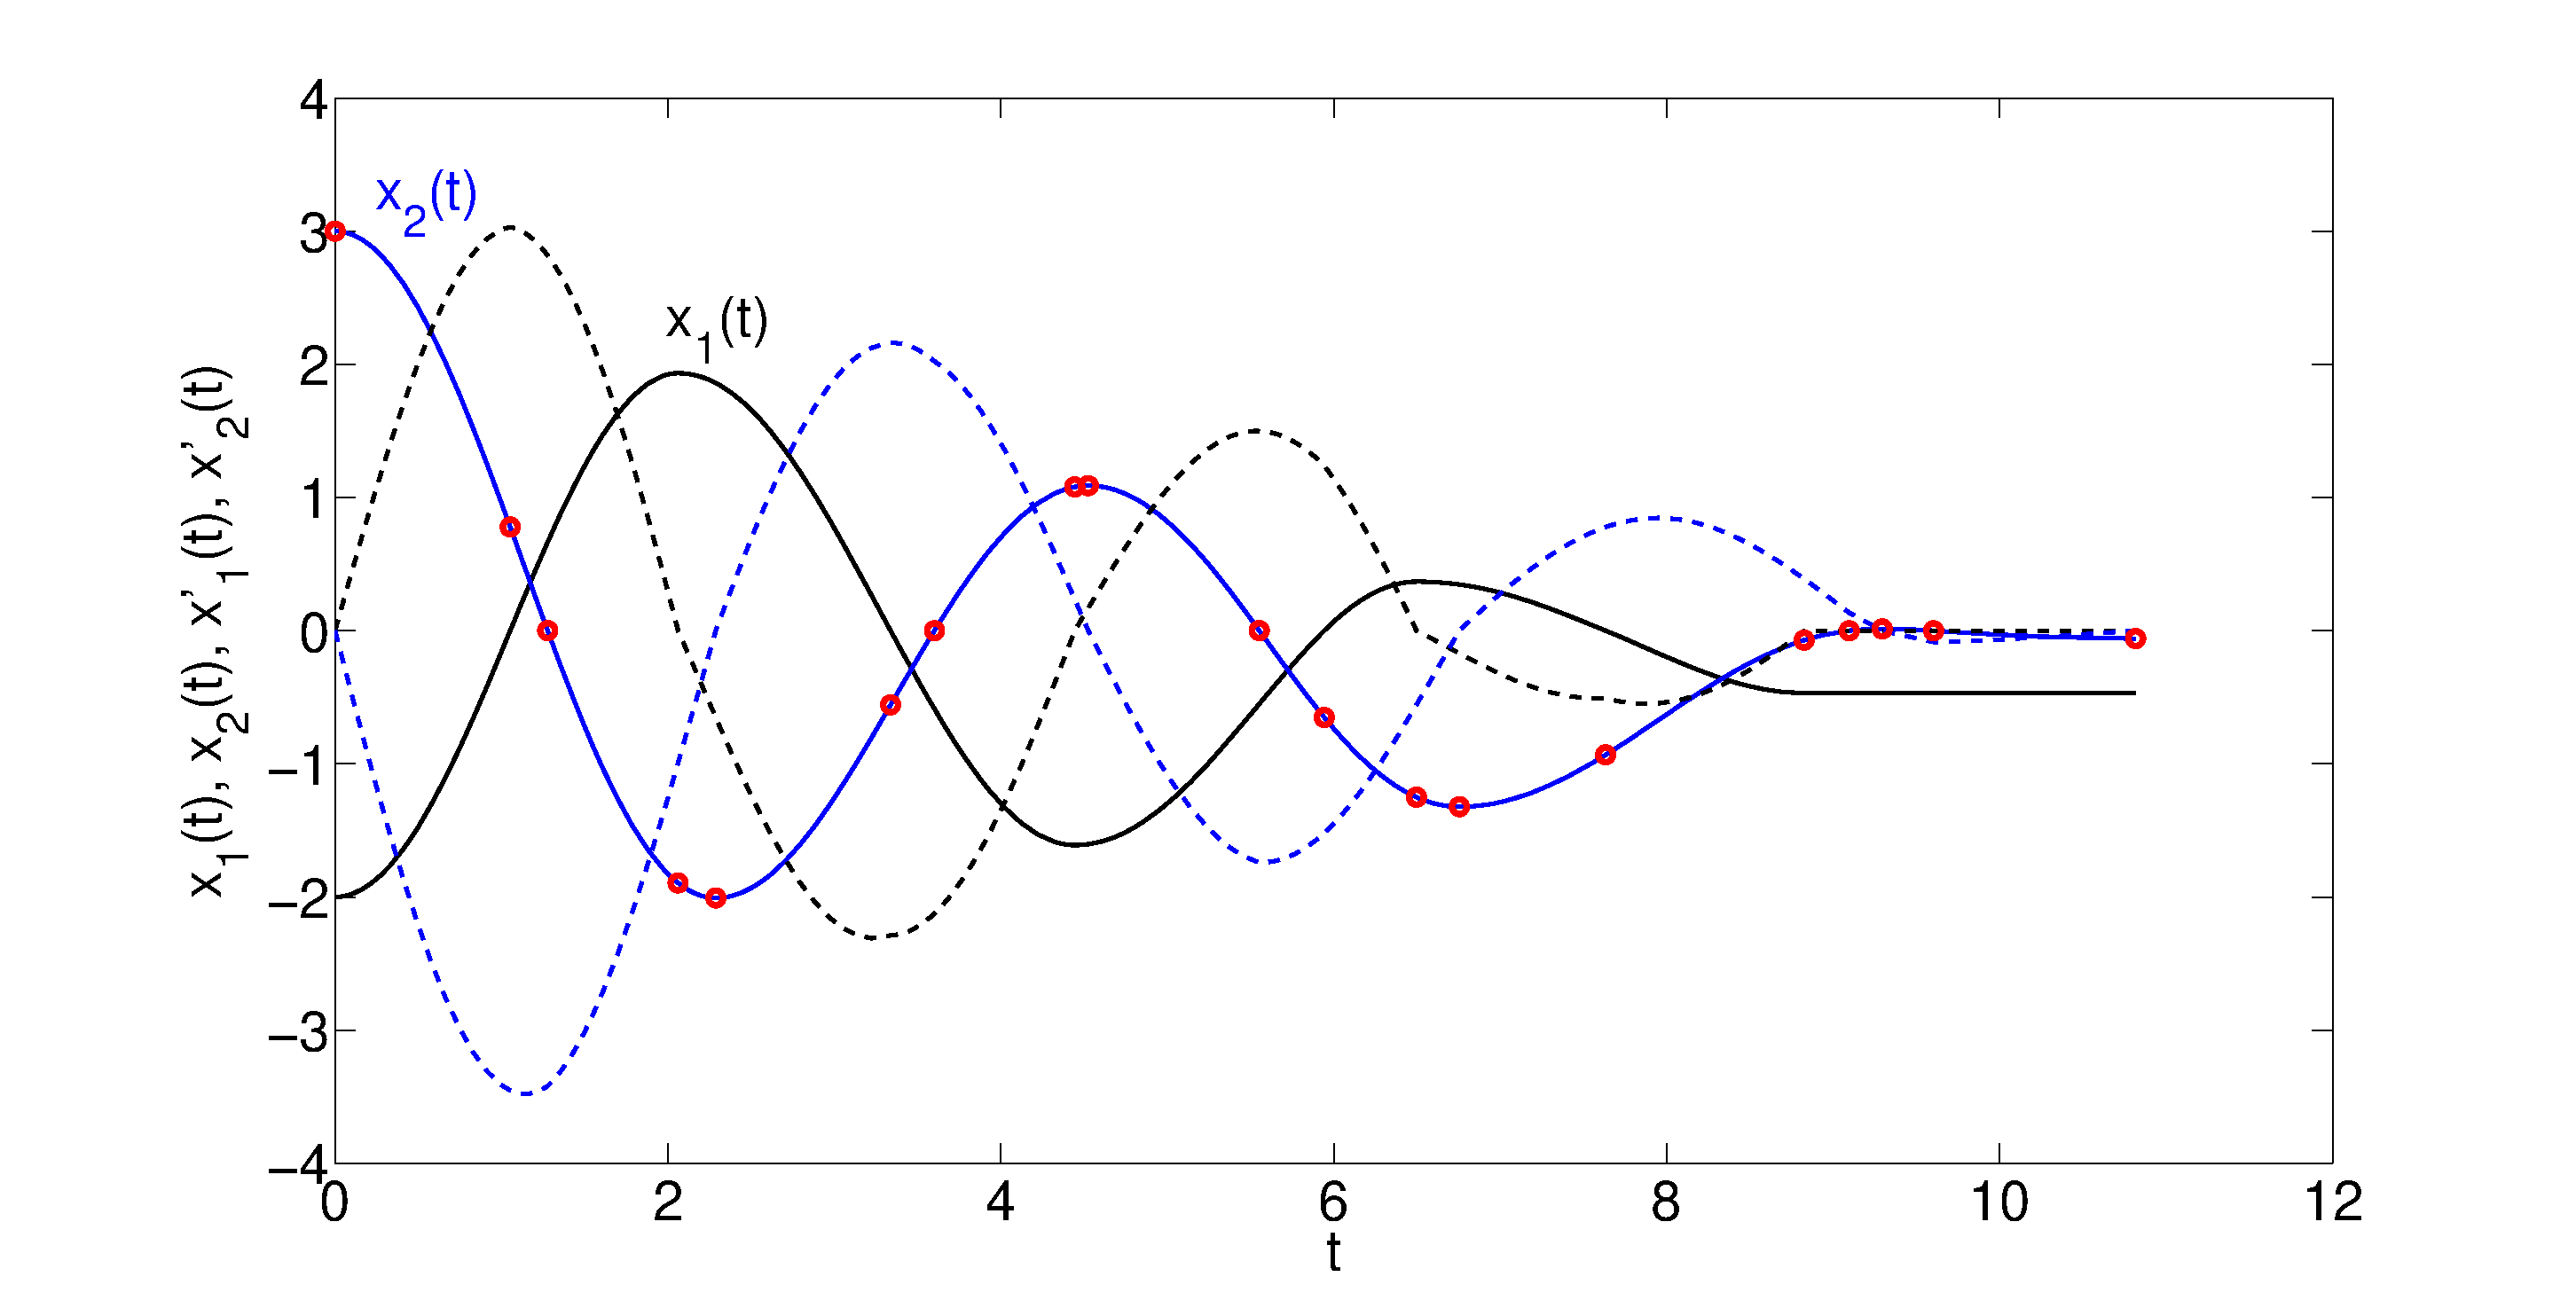
\includegraphics[width=14 true cm]{Example1}
}
\caption{Solution for Example 1}
\label{Example1}
\end{figure}


A Matlab code to integrate this problem with \texttt{disode45} can be

\bigskip

\begin{verbatim}
%
%  Call to disode45
%
 y0 = [-2;3;0;0];
 [tout,yout,tdis,ydis,idis,stats]=disode45(@fun, @gfun,[0,20], y0);
%
%  Definition of the vector field
%
 function f=fun1(t,y)
   E=1.0;
   if y(1) > 0
      mu1=1.0;
   else
      mu1=0.6;
   end
   if y(2) > 0
      mu2=0.2;
   else
      mu2=0.5;
   end
   f=[y(3);y(4);-E*(y(1)-y(2))-mu1*sign(y(3)); ...
                    -E*(y(2)-y(1))-mu2*sign(y(4))] ;
 end
%
%  Definition of the switching surfaces
%
 function [g,isterminal,direction]=gfun1(t,y)
   g=[y(3); y(4); y(1); y(2)];
   isterminal=[0;0;0;0];
   direction=[0;0;0;0];
 end
\end{verbatim}

Once the integration of this problem has concluded, the vectors \texttt{tdis}, \texttt{ydis} contain the switching point
and \texttt{idis} contain the following data

\begin{verbatim}
idis =

     1     3     4     1     2     3     4     1
     2     4     3     1     2     3    -1     4
     2     4    -2
\end{verbatim}

The elements of the vector \texttt{idis} indicate that the first switching point correspond to the first switching surface, the second one to the third surface and so on.  The positive elements mean that these discontinuities are transversal.
The negative ones mean that the solution enters into a sliding region.

The plots in Figure \ref{Example1} (without legends) can be obtained with the matlab order

\begin{verbatim}
plot(tout,yout(:,1),'k',tout,yout(:,2),'b', tout, ...
   yout(:,3),'k--',tout,yout(:,4),'b--',tdis,ydis(:,2),'ro');
\end{verbatim}

\item[Example 2]
In the second example (see \cite{Luo}) we consider a mass $m=1$ linked to a
wall by a spring of stiffness $k$
and a damper of viscous damping coefficient $r$. A external force $F=a_0 \cos(wt)$ is acting
upon the mass which is placed onto a belt that moves with velocity $v(t)= \cos(t) + 0.7$.
Therefore, a Coulomb friction force $F_C$ acts upon the mass.

\begin{center}
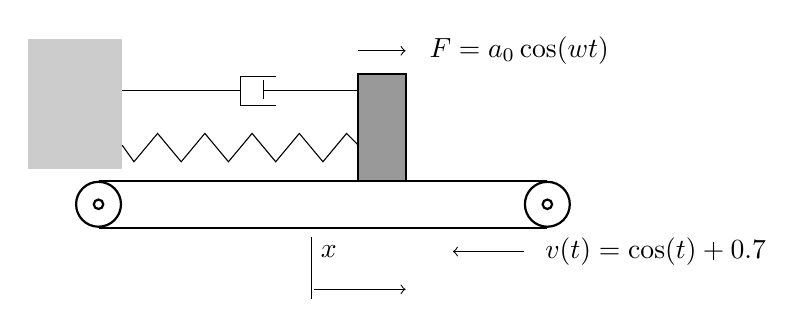
\begin{tikzpicture}[scale=3]
\draw (1.3,-0.3)-- (1.3,-0.04);
%\fill [black!20!white] (0.1,0.1) rectangle (2.3,0.2);
\draw (1.76,0.75) node [right] {$F=a_0 \cos(w t)$};
\draw [->] (1.5,0.75)-- (1.7,0.75);
\fill [black!40!white] (1.5,0.20) rectangle (1.7,0.65);
\draw [thick] (1.5,0.20) rectangle (1.7,0.65);
\fill [black!20!white] (0.1,0.25)rectangle (0.5,0.8);
\draw [thick] (0.4,0.20) -- (2.30,0.20);
\draw [thick] (0.4,0.0) -- (2.30,0.0);
\draw [thick] (0.4,0.10) circle (0.095);
\draw [thick] (0.4,0.10) circle (0.02);
\draw [thick] (2.3,0.10) circle (0.095);
\draw [thick] (2.3,0.10) circle (0.02);
\draw [->] (2.2,-0.1) -- (1.9,-0.1);
\draw (2.25,-0.1) node [right] {$v(t)= \cos(t)+0.7$};
\draw (1.3,-0.1) node [right] {$x$};
\draw [->] (1.31,-0.26)-- (1.7,-0.26);
\draw (0.5,0.35) -- (0.55,0.28) -- (0.65,0.40) -- (0.75,0.28) --
(0.85,0.40) --(0.95,0.28) -- (1.05,0.40) -- (1.15,0.28)-- (1.25,0.40) -- (1.35,0.28) --
(1.45,0.40) -- (1.50,0.35);
\draw (0.5,0.58) -- (1.0,0.58);
\draw (1.1,0.58) -- (1.5,0.58);
\draw (1.15,0.64) -- (1.0,0.64) -- (1.0,0.52) -- (1.15,0.52);
\draw (1.1,0.545) -- (1.1,0.625);
\end{tikzpicture}
\end{center}

This mechanical system is modelled by the non-smooth second order differential system
\[
\begin{cases}
x''  = -k x - 2 r x'+ a_0 \cos(w t) - F_C\; \hbox{sign}(x' - v(t) ),  & \\
F_C=0.4
\qquad
a_0=1, \quad r=0.2, \quad k=1, \quad w=0.7,
\\
v(t)=\cos (t) + 0.7,\\
x(0) = 3, x'(0)=0,  \vrule width 0pt height 16pt \\
t\in[0,30].
\end{cases}
\]
Expressed as a first order system with
two components $y_1(t)=x(t)$, $y_2(t)=x'(t)$, we have
\[
y'=\begin{pmatrix} y_1' \\y'_2 \end{pmatrix}=
\begin{pmatrix} y_2 \\ -k y_1 - 2 r y_2+ a_0 \cos(w t) - F_C\; \hbox{sign}(y_2 - v(t) )
\end{pmatrix} = f(t,y)
\]

\medskip

Clearly the vector field $f(t,y)$ is non smooth at points where $x'(t)=y_2(t)=v(t)$.
Then, we have one switching surface  $g(y)=y_2-v(t)$, that depends on $y_2$
and also on $v(t)$.

The solution $x(t)$ and its derivative $x'(t)$  are depicted in the  upper plot of Figure \ref{Example2}.  The discontinuity points (where the second derivative $x''(t)$ is not continuous) are indicated by means of small circles.
To visualize the sliding regions, we give in the down plot of Figure \ref{Example2} the function $x'(t)-v(t)$.
The sliding regions correspond to the intervals at which the functions vanishes.

\begin{figure}[!h]
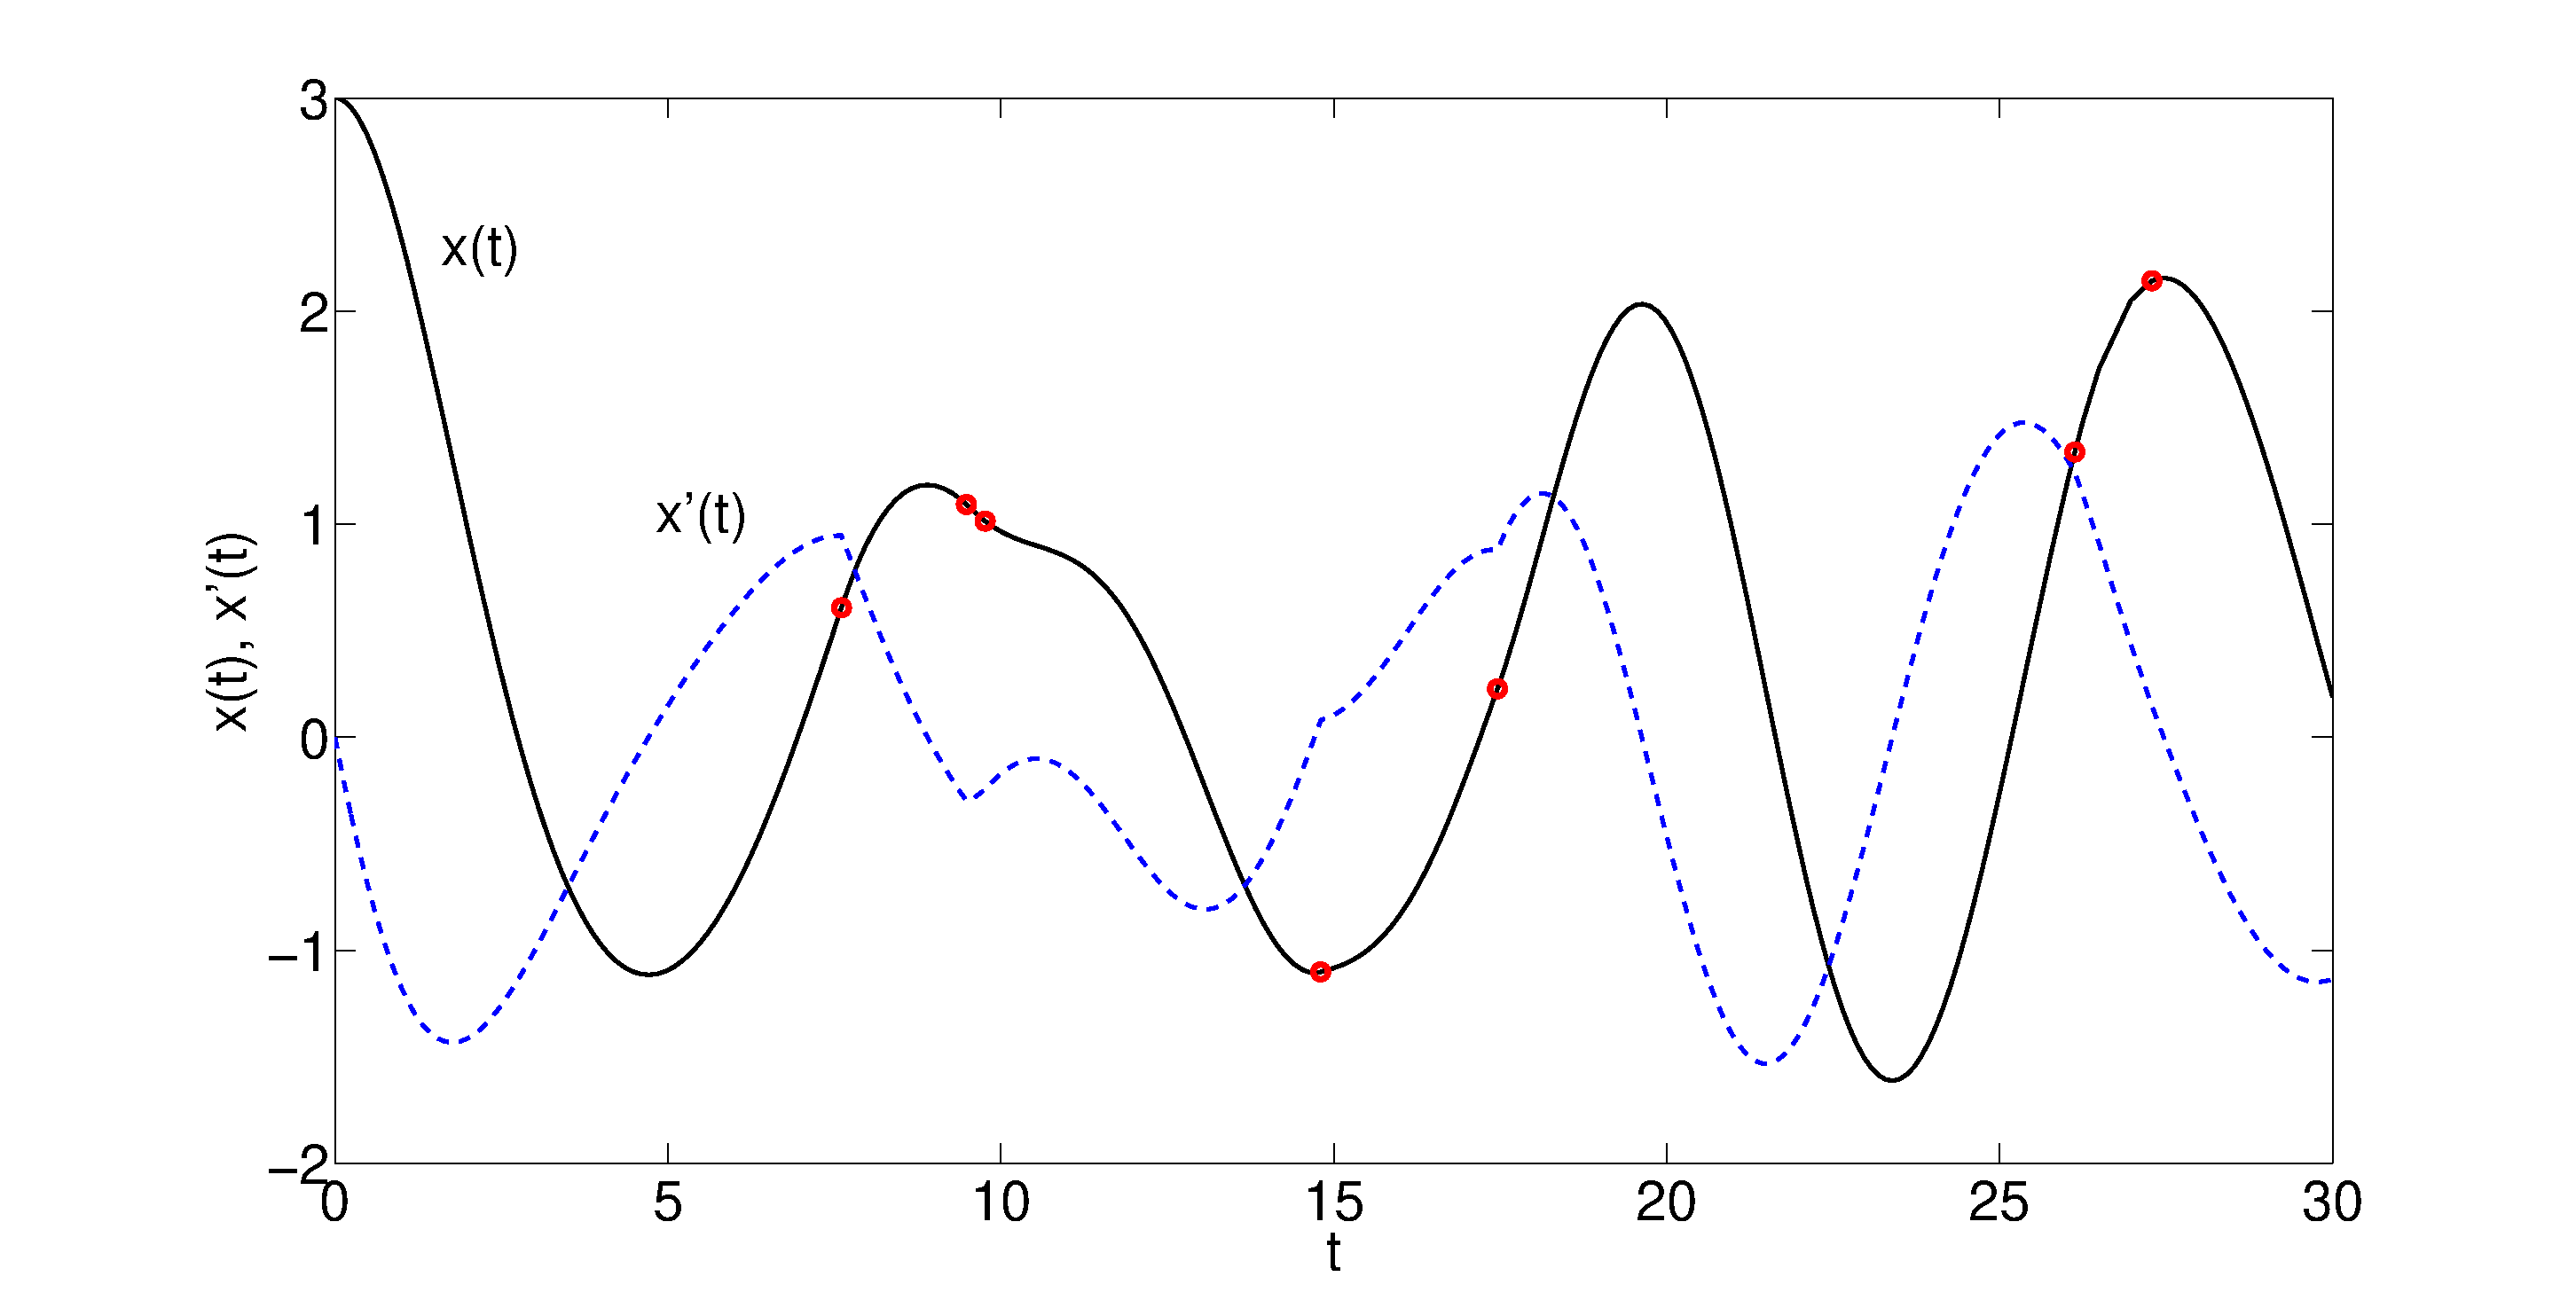
\includegraphics[width=12 true cm]{Example2} \\
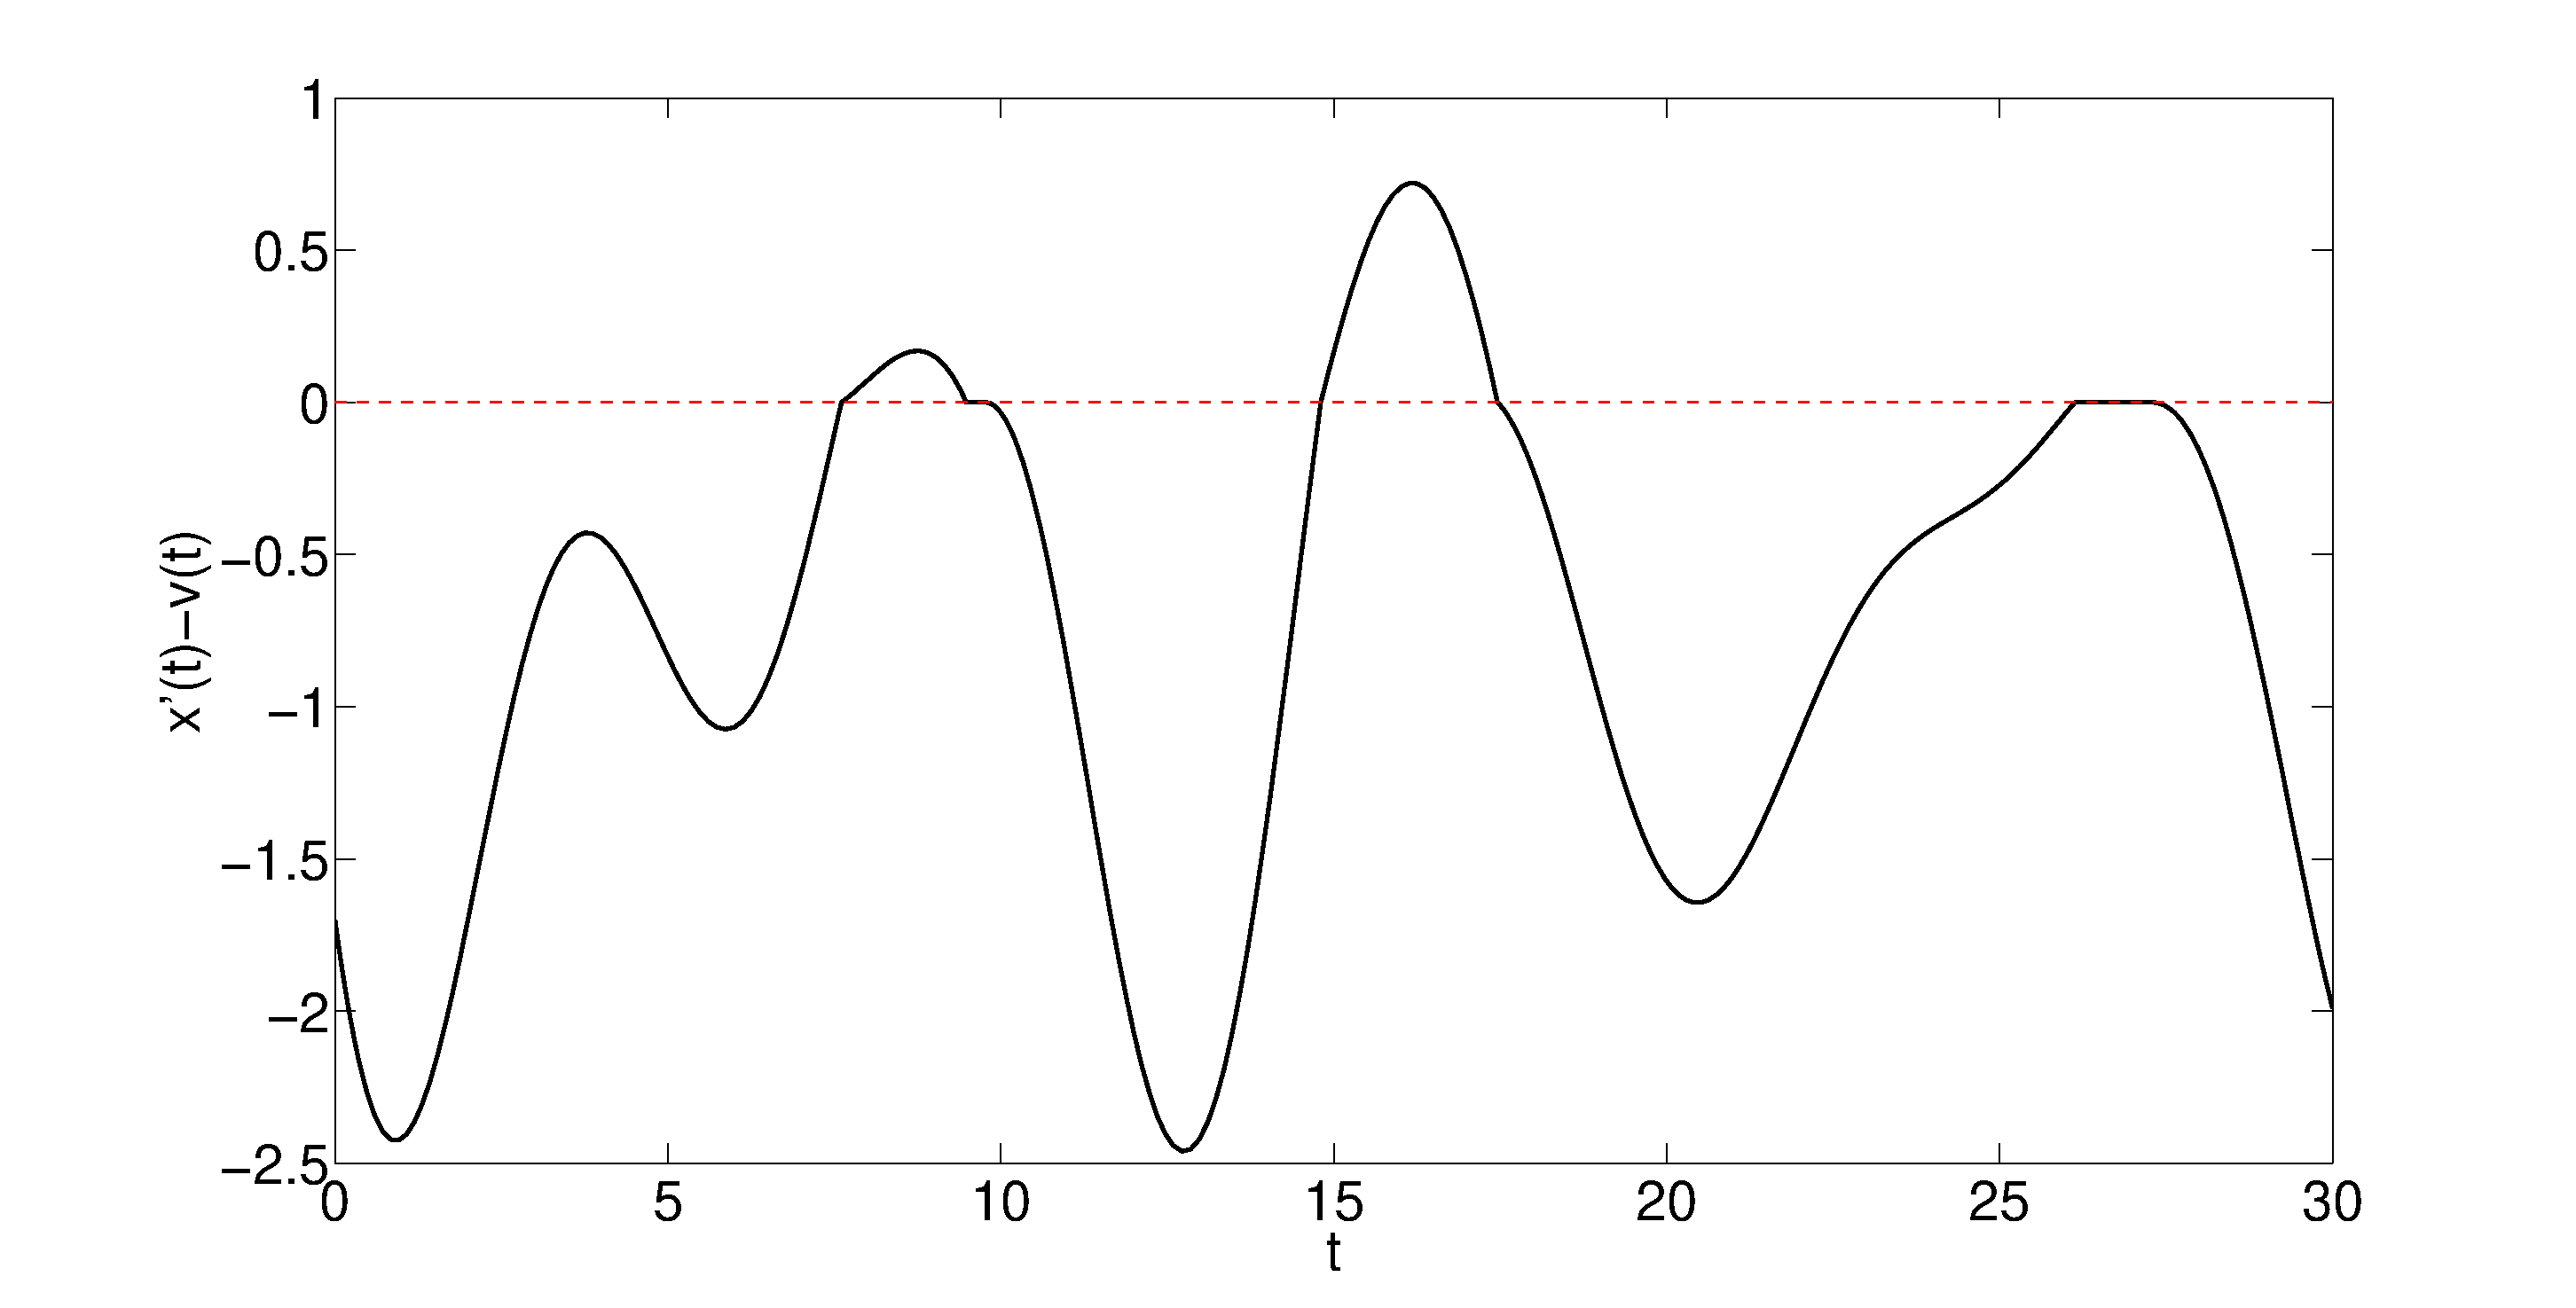
\includegraphics[width=12 true cm]{Example2-sliding}
\caption{Example 2, Solution (top) and  Sliding regions (dowm)}
\label{Example2}
\end{figure}

The solution, with the considered initial conditions,
passes first through a transversal discontinuity, then  it enters a sliding
region for a short time until it exits it, then it passes through two transversal discontinuities and then
it enters into another sliding region.

A Matlab code to integrate this problem with \texttt{disode45} can be

\bigskip

\begin{verbatim}
%
%  Call to disode45
%
 y0 = [3;0];
 [tout,yout,tdis,ydis,idis,stats]=disode45(@fun, ...
                                    @gfun,[0,30], y0);
%
%  Definition of the vector field
%
 function f=fun(t,y)
      k=1.0;
      r=0.2;
      a0=1.0;
      w=0.7;
      Fc=0.4;
      v=cos(t)+0.7;
      f=[y(2);-k*y(1)-2*r*y(2)+a0*cos(w*t)-Fc*sign(y(2)-v)];
 end
%
%  Definition of the switching surfaces
%
 function [g,isterminal,direction]=gfun(t,y)
    v=cos(t)+0.7;
    g=y(2)-v;
    isterminal=0;
    direction=0;
 end
\end{verbatim}

Once the integration of this problem concludes, the vectors tdis, ydis
and idis contain the following data

\begin{verbatim}
tdis =

    7.6056    9.4835    9.7653   14.8051   17.4589   26.1318   27.2913

ydis =

    0.6072    0.9459
    1.0923   -0.2983
    1.0143   -0.2426
   -1.1013    0.0806
    0.2269    0.8792
    1.3390    1.2411
    2.1418    0.1455

idis =

     1    -1    -1     1     1    -1    -1
\end{verbatim}

In this case, the second element of \texttt{idis} equal to $-1$ means that the solution
enters into a sliding region, and the third one, also $-1$, means that the solution
exits from the sliding region.  The same happens with the last two elements.

The plots in Figure \ref{Example2} (without legends) can be obtained with the matlab orders

\begin{verbatim}
plot(tout,yout(:,1),'k',tout,yout(:,2),'k--', tdis, ...
                                          ydis(:,1),'ro');
plot(tout,yout(:,2)-0.7-cos(tout)',[0,30],[0,0],'r');
\end{verbatim}


\item[Example 3]
In the third example (see A. Luo \cite[pp. 115]{Luo}) we consider two masses $m_1$ and $m_2$ linked to a
wall by springs of stiffness $k_1, k_2$ respectively
and dampers of viscous damping coefficients $r_1, r_2$. A external force $F=a_0 \cos(wt)$ is acting
upon the mass $m_1$.  Mass $m_1$ is placed into a hole in mass $m_2$ so that the masses
can hit each other as depicted in Figure \ref{system3}.

\begin{figure}[h]
\begin{center}
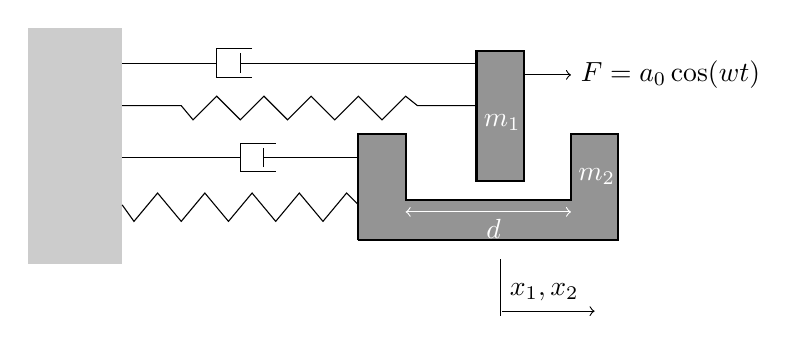
\begin{tikzpicture}[scale=3]
%\fill [black!20!white] (0.1,0.1) rectangle (2.3,0.2);
\draw (2.4,0.9) node [right] {$F=a_0 \cos(w t)$};
\draw [->] (2.2,0.9)-- (2.4,0.9);
\fill [black!42!white] (1.5,0.20)--(1.5,0.65)-- (1.7,0.65)--(1.7,0.37)--(2.4,0.37)--(2.4,0.65)-- (2.6,0.65)--(2.6,0.2)--(1.5,0.20);
\draw [thick] (1.5,0.20)--(1.5,0.65)-- (1.7,0.65)--(1.7,0.37)--(2.4,0.37)--(2.4,0.65)-- (2.6,0.65)--(2.6,0.2)--(1.5,0.20);
\fill [black!42!white] (2.0,0.45)rectangle (2.2,1.0);
\draw [thick] (2.0,0.45)rectangle (2.2,1.0);
\fill [black!20!white] (0.1,0.10)rectangle (0.5,1.1);
\draw [white] (1.99,0.7) node [right] {$m_1$};
\draw [white] (2.39,0.47) node [right] {$m_2$};
\draw (2.1,-0.02) node [right] {$x_1, x_2$};
\draw [white,<->] (1.7,0.32)-- (2.4,0.32);
\draw [white] (2.0,0.25) node [right] {$d$};
\draw [->] (2.11,-0.10)-- (2.5,-0.10);
\draw (2.1,-0.12)-- (2.1,0.12);
\draw (0.5,0.35) -- (0.55,0.28) -- (0.65,0.40) -- (0.75,0.28) --
(0.85,0.40) --(0.95,0.28) -- (1.05,0.40) -- (1.15,0.28)-- (1.25,0.40) -- (1.35,0.28) --
(1.45,0.40) -- (1.50,0.35);
\draw (0.5,0.55) -- (1.0,0.55);
\draw (1.1,0.55) -- (1.5,0.55);
\draw (1.15,0.61) -- (1.0,0.61) -- (1.0,0.49) -- (1.15,0.49);
\draw (1.1,0.51) -- (1.1,0.59);
\draw (0.5,0.95) -- (0.9,0.95);
\draw (1.0,0.95) -- (2.0,0.95);
\draw (1.05,1.01) -- (0.9,1.01) -- (0.9,0.89) -- (1.05,0.89);
\draw (1.0,0.908) -- (1.0,0.992);
\draw (0.5,0.77)--(0.75,0.77) -- (0.80,0.71) -- (0.90,0.81) -- (1.00,0.71) --
(1.10,0.81) --(1.20,0.71) -- (1.30,0.81) -- (1.40,0.71)-- (1.50,0.81) -- (1.60,0.71) --
(1.70,0.81) -- (1.75,0.77)--(2.0,0.77);
\end{tikzpicture}
\end{center}
\caption{Example 3}
\label{system3}
\end{figure}

Whenever both masses have no contact, that is, $y_1-y_2 >d/2$
or $y_2-y_1 > d/2$,
this mechanical system is modelled by the differential system
\begin{equation}
\label{nonsticking}
\begin{array}{l}
m_1 x_1''  = -k_1 x_1 - r_1 x_2'+ a_0 \cos(w t)+b_0 \\
m_2 x_2''  = -k_2 x_2 - r_2 x_2'
\end{array}
\end{equation}
When the masses hit each other, $|x_1-x_2|=d/2$, the behaviour of the system depends
on their velocity.  If they are different, $x_1' \ne x_2'$, we have a switching point
in which the vector field does not change but the initial conditions of the system
change from $(x_1,x_2,x_1', x_2')$ to $(\hat x_1,\hat x_2,\hat x_1', \hat x_2')$
according to the following formulas
\[
\begin{array}{l}
\hat x_1= x_1, \\
 \hat x_2=x_2, \\[8pt]
\hat x_1'= \dfrac{m_1-m_2 e}{m_1+m_2}\;x_1'+\dfrac{(1+e)m_2}{m_1+m_2}\;x_2', \\[8pt]
\hat x_2'= \dfrac{m_2-m_1 e}{m_1+m_2}\; x_1'+\dfrac{(1+e)m_1}{m_1+m_2}\;x_2'.
\end{array}
\]
If the masses hit with the same velocity, the system enters
into a sticking region that is governed by the differential system
\[
\begin{array}{l}
(m_1+ m_2) x_1''  = -(k_1+k_2) x_1 - (r_1+r_2) x_1')+
\dfrac{k_2 d}{2}+ a_0 \cos(w t)+b_0,  \\[10pt]
(m_1+ m_2) x_2'' =  -(k_1+k_2) x_2 - (r_1+r_2) x_2')-
\dfrac{k_1 d}{2}+ a_0 \cos(w t)+b_0,
\end{array}
\]
if $x_1=x_2+d/2$ or
\[
\begin{array}{l}
(m_1+ m_2) x_1''  = -(k_1+k_2) x_1 - (r_1+r_2) x_1')-
\dfrac{k_2 d}{2}+ a_0 \cos(w t)+b_0,  \\[10pt]
(m_1+ m_2) x_2'' =  -(k_1+k_2) x_2 - (r_1+r_2) x_2')+
\dfrac{k_1 d}{2}+ a_0 \cos(w t)+b_0,
\end{array}
\]
if $x_2=x_1+d/2$.

Note that in this region, since $|x_1-x_2|=d/2$, it holds $x''_1(t) = x''_2(t)$
and $x'_1(t)=x_2(t)$.
The system stays in this region while the forces per unit mass, that act upon each
mass
\[
\begin{array}{l}
u_1= \dfrac{F_1}{m_1}=-\dfrac{r1}{m1} x_1'-\dfrac{k1}{m1} x_1+\dfrac{b_0+a_0 \cos(w t)}{m1} \\[10pt]
u_2= \dfrac{F_2}{m_2}=-\dfrac{r2}{m2} x_2'-\dfrac{k2}{m2} x_2
\end{array}
\]
satisfy  $x_1-x_2=d/2$ and $u_1 \ge u_2$ or well
$x_2-x_1=d/2$ and $u_2 \ge u_1$.  In other case, the systems goes back to the
non sticking evolution and equations \eqref{nonsticking} govern the evolution
of the system.

With the above considerations, and defining the state vector by
$y(t)=(y_1(t), y_2(t), y_3(t), y_4(t))^T = (x_1(t), x_2(t), x_1'(t), x_2'(t))^T$
the system can be modelled by the non smooth system
\[
y'(t)= A(t) y(t) + b(t),
\]
with
\[
A(t)=\begin{cases}
\begin{pmatrix}0 & 0 & 1 & 0 \\ 0 & 0 & 0 & 1 \\
-\dfrac{k_1+k_2}{m_1+m_2} & -\dfrac{r_1+r_2}{m_1+m_2} & 0 & 0 \\[10pt]
-\dfrac{k_1+k_2}{m_1+m_2} & -\dfrac{r_1+r_2}{m_1+m_2} & 0 & 0\end{pmatrix},
&
\begin{array}{l}
\hbox{ if }  y_1-y_2 \ge d/2 \hbox{ and } u_1 \ge u_2 \\
\hbox{ or }
y_2-y_1 \ge d/2 \hbox{ and } u_2 \ge u_1
\end{array}
\\[50pt]
\begin{pmatrix}0 & 0 & 1 & 0 \\ 0 & 0 & 0 & 1 \\
-\dfrac{k_1}{m_1} & -\dfrac{r_1}{m_1} & 0 & 0 \\ -\dfrac{k_2}{m_2} & -\dfrac{r_2}{m_2} & 0 & 0\end{pmatrix},
&  \hbox{ otherwhise. }
\end{cases}
\]

\[
b(t)=\begin{cases}
\begin{pmatrix}0\\0\\ \dfrac{k_2 d/2}{m_1+m_2}+\dfrac{a_0 \cos(w t)}{m_1+m_2}  \\[10pt]
\dfrac{-k_1 d/2}{m_1+m_2}+\dfrac{a_0 \cos(w t)}{m_1+m_2}  \end{pmatrix},
&  \hbox{ if }  y_1-y_2 \ge d/2 \hbox{ and } u_1 \ge u_2
\\[50pt]
\begin{pmatrix}0\\0\\ \dfrac{-k_2 d/2}{m_1+m_2}+\dfrac{a_0 \cos(w t)}{m_1+m_2}  \\[10pt]
\dfrac{k_1 d/2}{m_1+m_2}+\dfrac{a_0 \cos(w t)}{m_1+m_2}  \end{pmatrix},
&  \hbox{ if } y_2-y_1 \ge d/2 \hbox{ and } u_2 \ge u_1
\\[50pt]
\begin{pmatrix}0\\0\\ \dfrac{b_0}{m1}+\dfrac{a_0}{m1}\cos(w t) \\0  \end{pmatrix},
&  \hbox{ otherwhise }
\end{cases}
\]

In this example we have taken
\[
r_1=0.6, \quad r_2=0.6, \quad k_1=30, \quad k_2=20, \quad  a_0=1, \quad w=0.7,
\quad b_0=35
\]
and as initial conditions
\[
y_1(0) = 0.2, y_2(0)=0.3, y_1'(0)=0, y_2'0)=0, \quad
t\in[0,10].
\]

\medskip

The vector field $f(t,y)$ is non smooth at points where $y_1-y_2=d/2$,
when $y_2-y_1=d/2$.
Starting with the selected initial conditions, the system evolves smoothly until the masses hit. Then,
a series of hits happen repeatedly, each time after less time.  After a finite time, but infinite hits,
the masses hit with the same velocity and the system enters into a sticking region.  After some time, the
system leaves this region and the behaviour repeats the same process.  In the bottom plot of
Figure \ref{Example3} we depict the function $x_1(t)-x_2(t)$.  The points where
$x_1(t)-x_2(t)=0.5$ correspond to points where the masses hit, and the intervals where
$x_1(t)-x_2(t)$ correspond to sticking regions. In the top plot of Figure \ref{Example3}
we show the solution $x_1(t), x_2(t)$ against time $t$. again, the discontinuity points
are indicated by means of small circles.

\begin{figure}[!h]
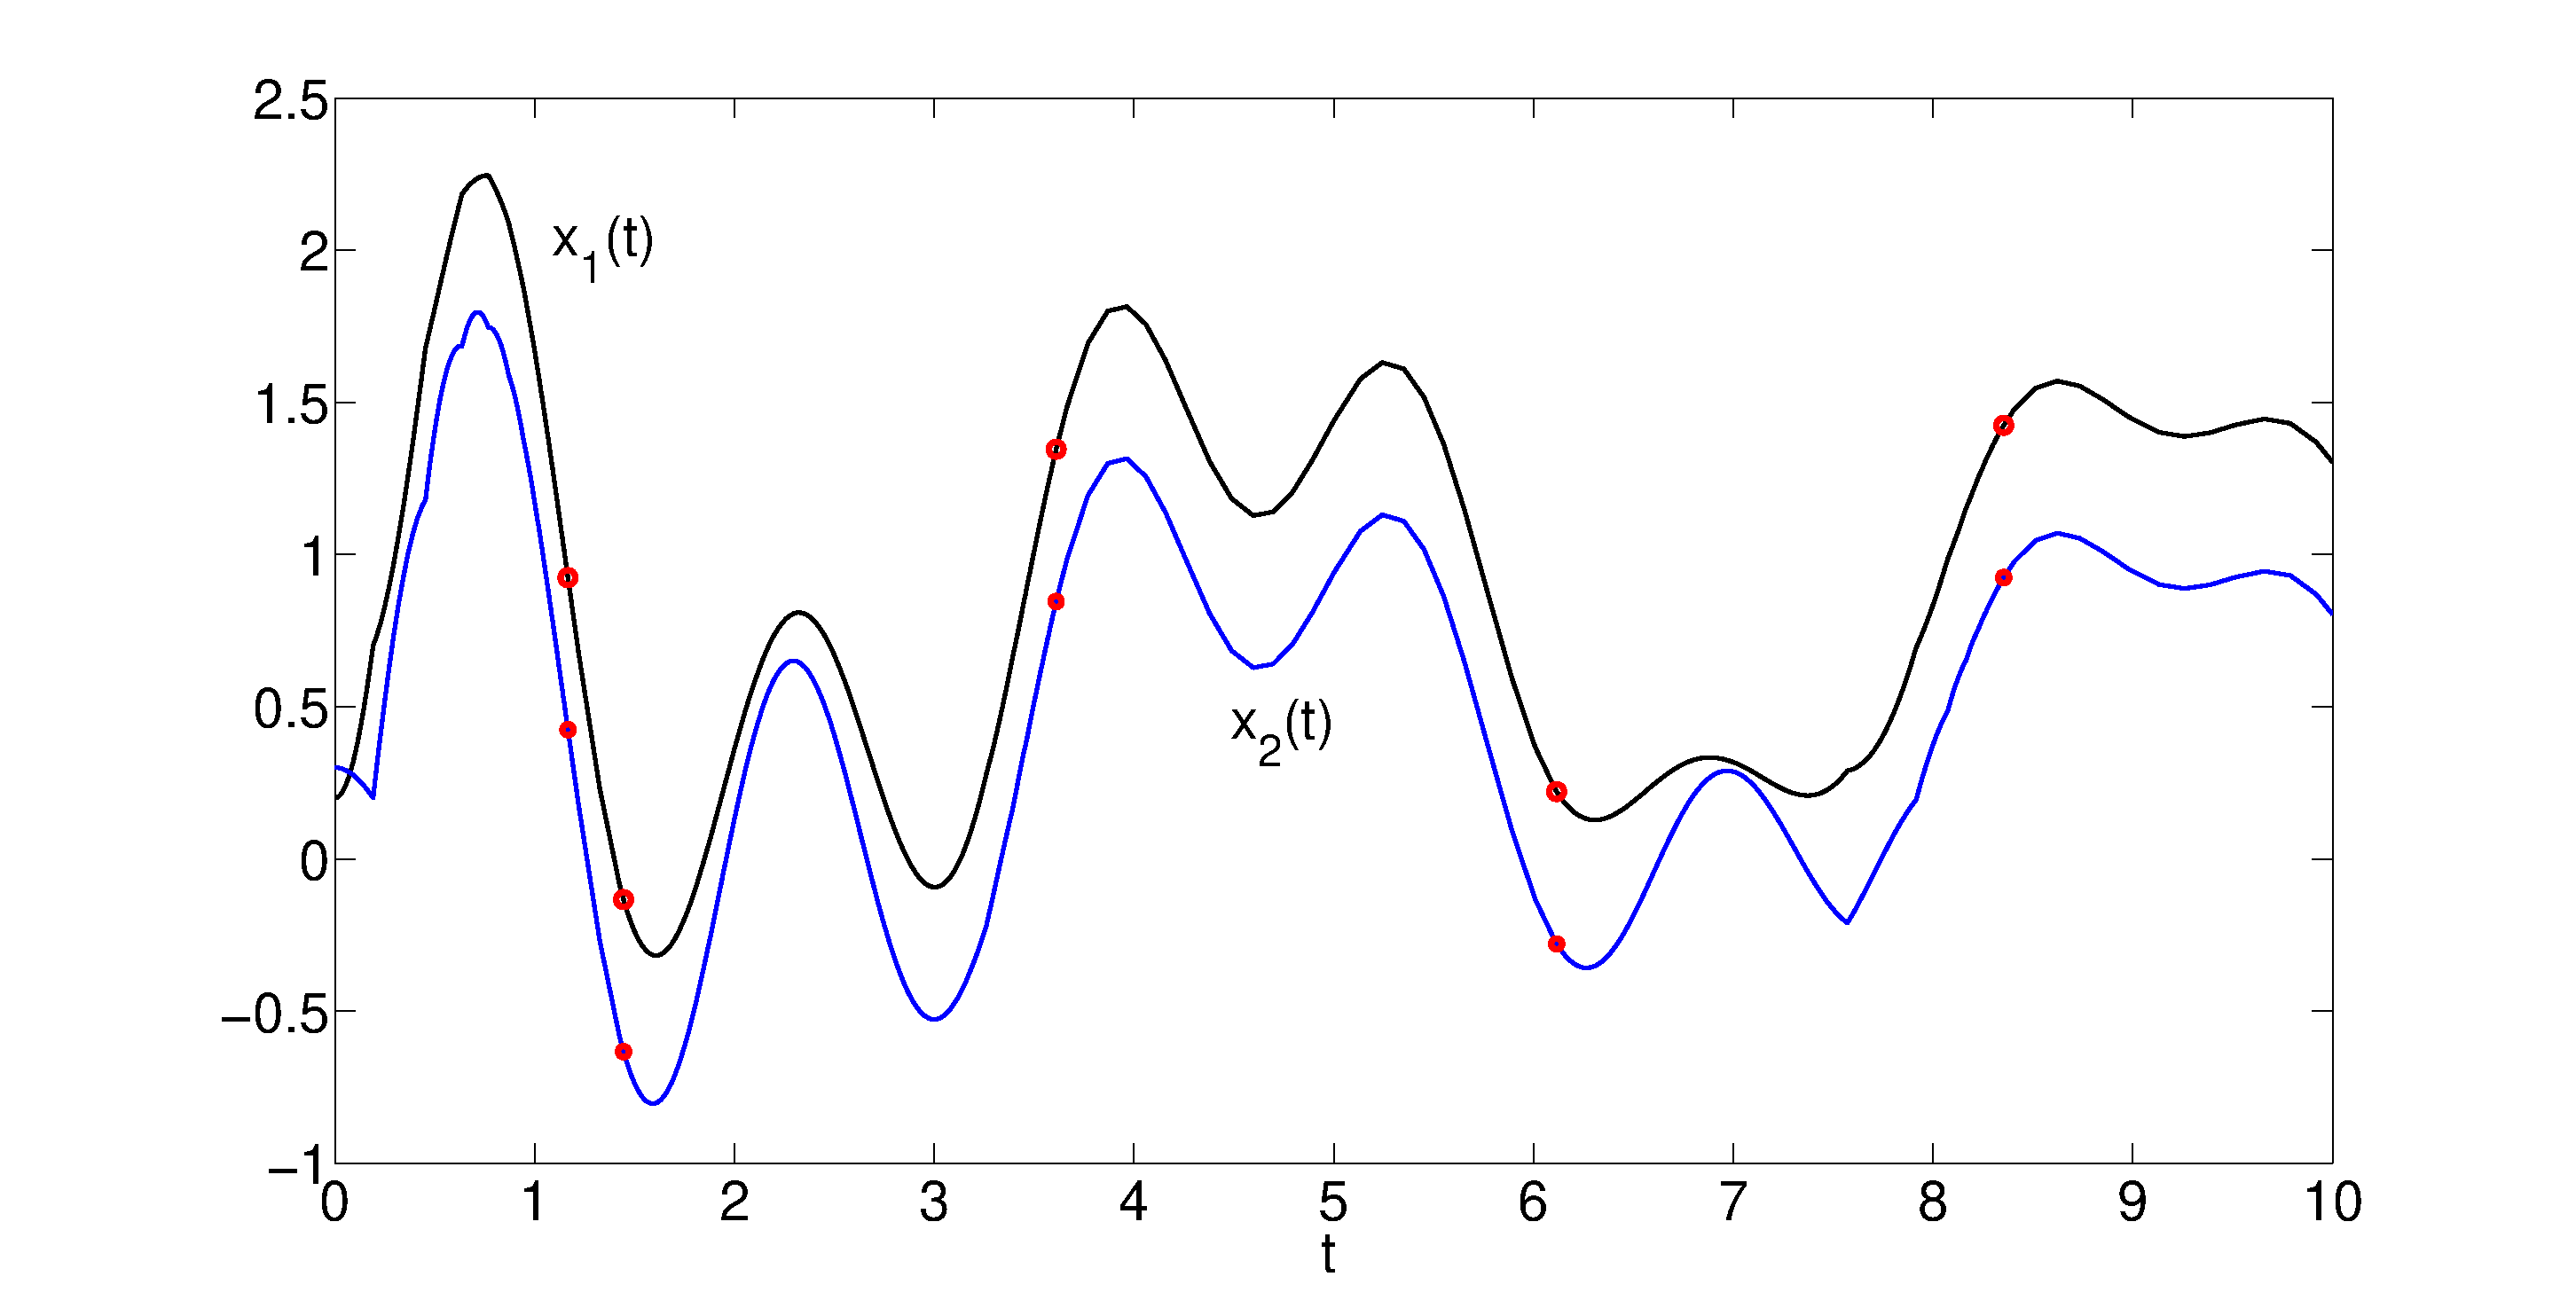
\includegraphics[width=12 true cm]{Example3} \\
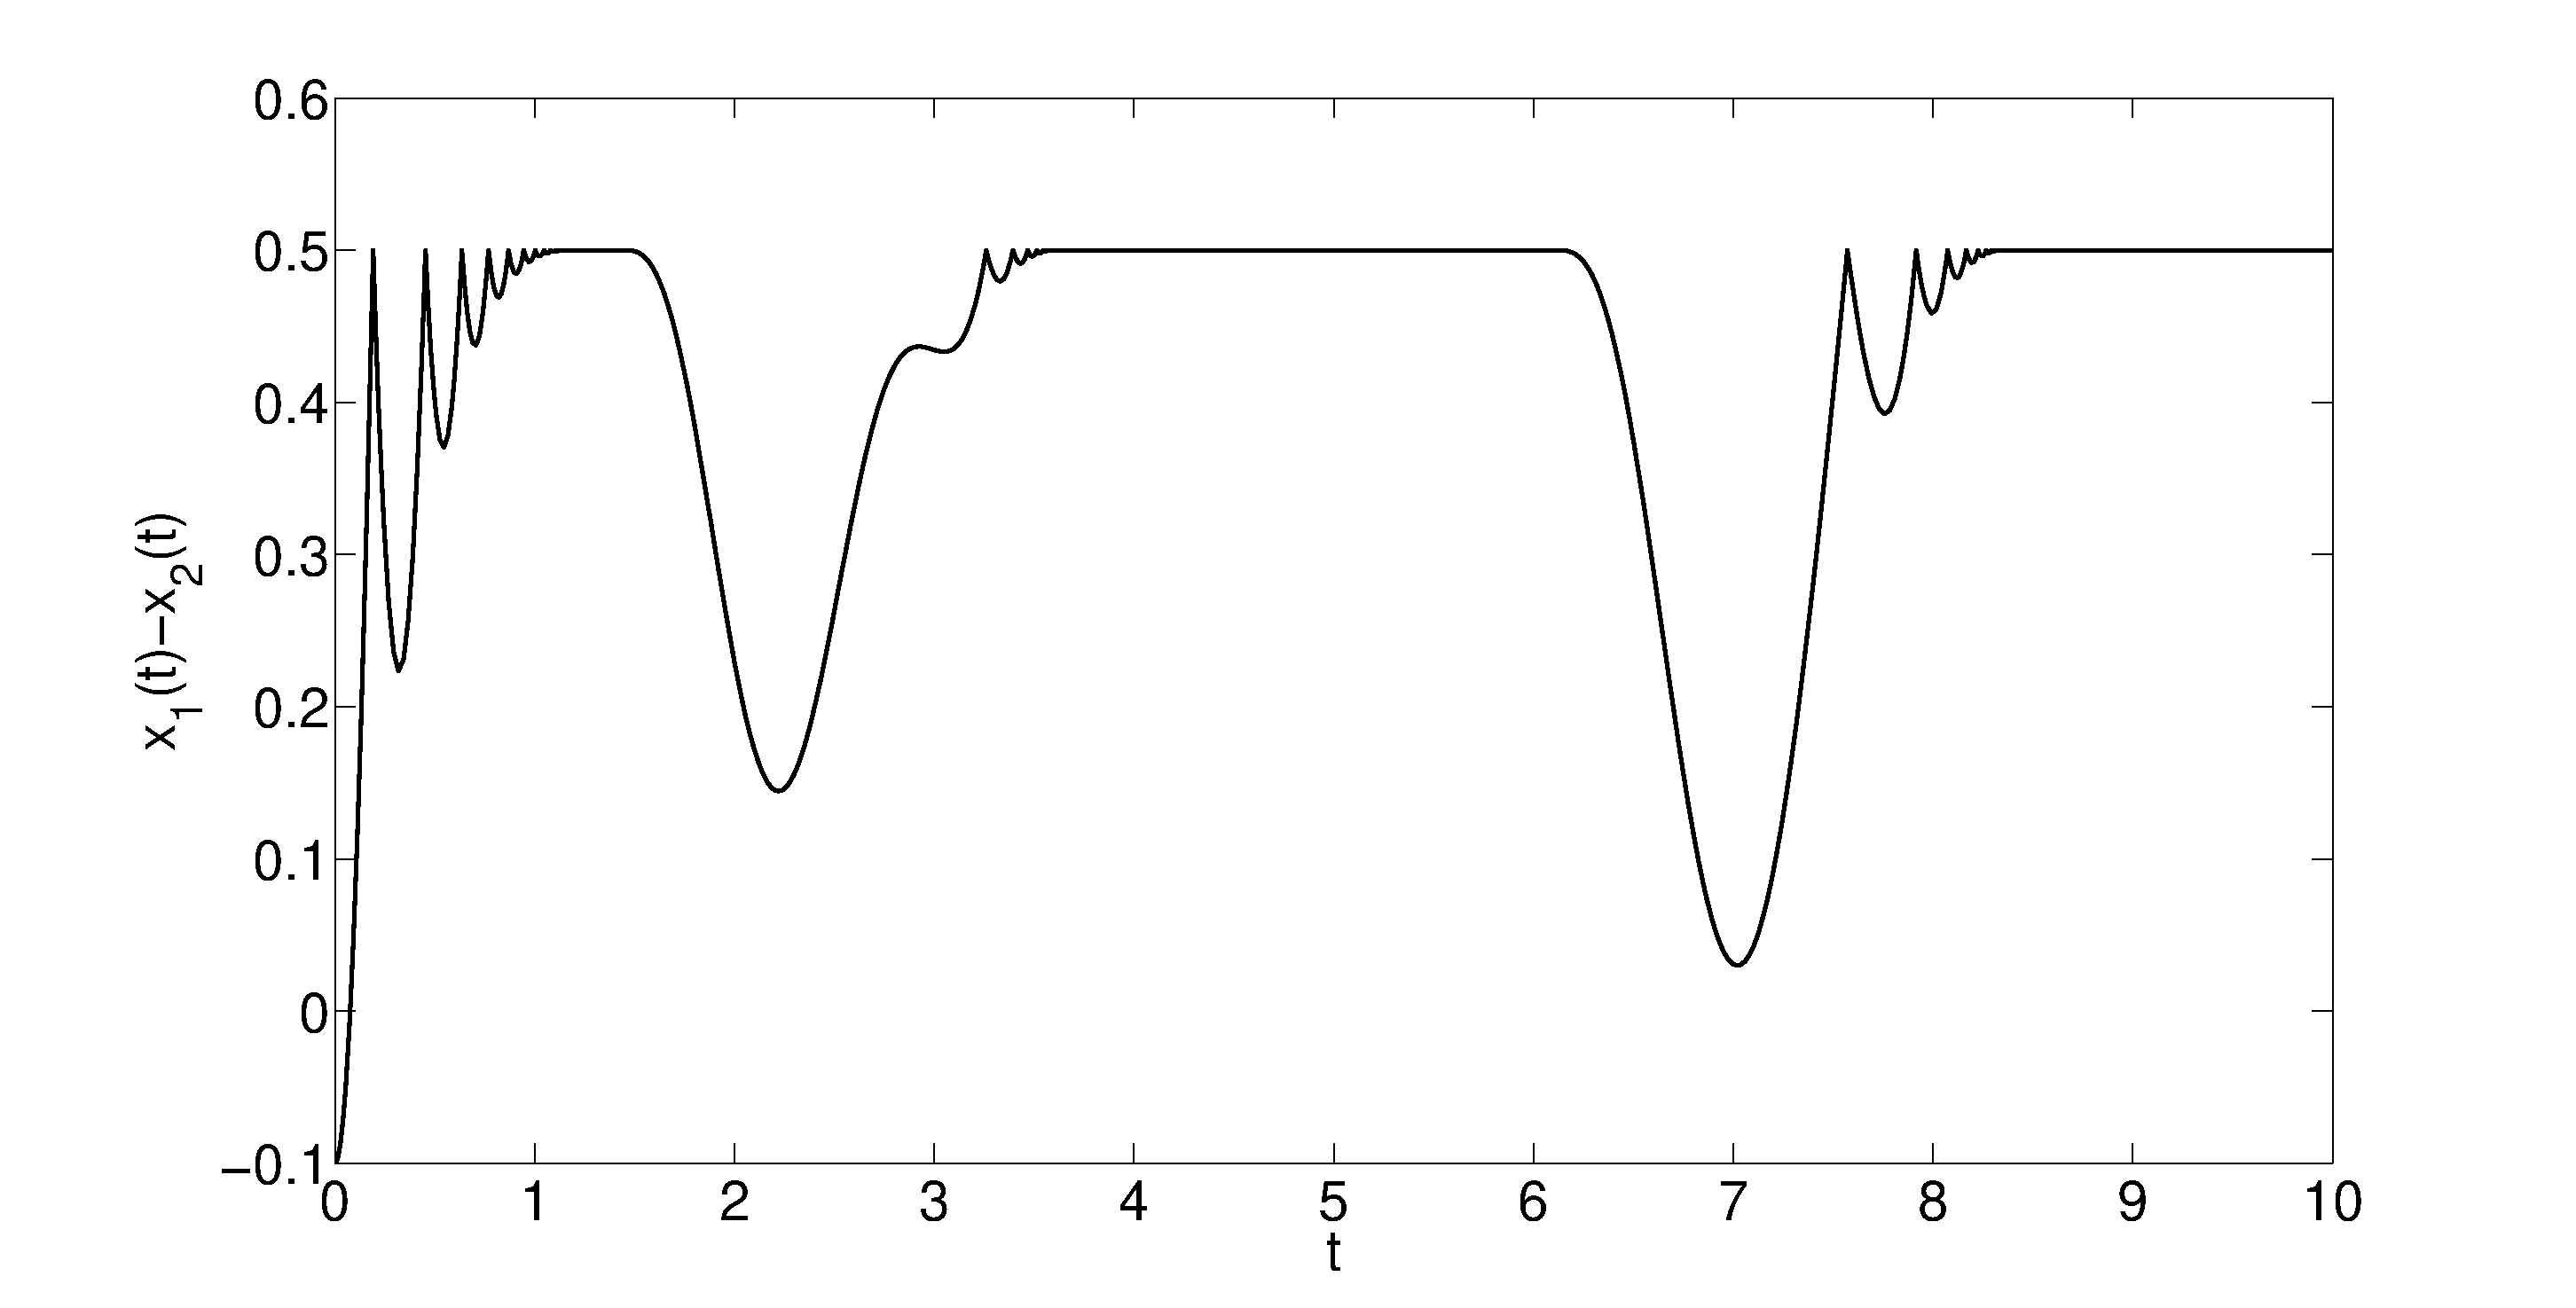
\includegraphics[width=12 true cm]{Example3-sliding}
\caption{Example 3, Solution (top) and  Sliding regions (bottom)}
\label{Example3}
\end{figure}

This problem has two specially complicated characteristics.  On one side, the initial point of a sticking region
is in fact a accumulation point of discontinuities, and in theory to attain it we should detect
an infinity number of switching points.  To solve this, the start of the sticking region can be
assumed when $|x_1 -x_2|=d/2$ and $|x'_1(t)-x'_2(t)| < c$ for some small value of $c$.  In our numerical
computations we ha taken $c=10^{-6}$.
The second special characteristic is that at the moment the sticking region is attained the trajectory of
the system is tangent to the switching surface.  Thus, for the surface $g_1(y)=y_1-y_2-d/2=0$,
the gradient vector is $\nabla g_1=(1,-1,0,0)^T$ and the sticking region is attained at a point
$y^*=(y_2 +d/2, y_2, y_4, y_4)^T$.  At this point, the vector field has a value
$f(t,y^*)= (y_4, y_4, -(k_1/m_1) y_1, -(k_2/m_2)/y_2)^T $ and clearly,
$\nabla g_1(y^*) \cdot f(t,y^*)=0$.
This means that the numerical approximation can not be reliable, in the sense that a small error
in the approximation of the solution can lead to a great error in the time $t$ at which the
solution starts the sticking region.

A Matlab code to integrate this problem with \texttt{disode45} can be

\bigskip

\begin{verbatim}
%
%  Call to disode45
%

 options=disodeset('RelTol',1.e-5,'AbsTol',1.e-5, ...
                        'ActionSwitch',@actionatswitch);
 y0 = [0.2;0.3;0;0];
 [tout,yout,tdis,ydis,idis,stats]=disode45(@fun, @gfun, ...
                                       [0,10], y0,options);
%
%  Definition of the vector field
%
 function f=fun(t,y)
    m1=2;
    m2=1;
    r1=0.6;
    r2=0.6;
    k1=30;
    k2=20;
    a0=30;
    b0=35;
    d=1.0;
    ee=0.7;
    w=1.38;
    u1=-(r1/m1)*y(3)-(k1/m1)*y(1)+b0/m1+(a0/m1)*cos(w*t);
    u2=-(r2/m2)*y(4)-(k2/m2)*y(2);
    if y(1)-y(2)>= d/2 && u1>=u2,
       f=[y(3);y(3); ...
          -((r1+r2)/(m1+m2))*y(3)-((k1+k2)/(m1+m2))*y(1)+ ...
          b0/(m1+m2)+(k2*d/(2*m1+2*m2))+(a0/(m1+m2))*cos(w*t);...
          -((r1+r2)/(m1+m2))*y(3)-((k1+k2)/(m1+m2))*y(1)+ ...
          b0/(m1+m2)+(k2*d/(2*m1+2*m2))+(a0/(m1+m2))*cos(w*t)];
    elseif y(2)-y(1)>= d/2 && u2>=u1,
       f=[y(3);y(3); ...
          -((r1+r2)/(m1+m2))*y(3)-((k1+k2)/(m1+m2))*y(1)+ ...
          b0/(m1+m2)-(k2*d/(2*m1+2*m2))+(a0/(m1+m2))*cos(w*t);...
          -((r1+r2)/(m1+m2))*y(3)-((k1+k2)/(m1+m2))*y(1)+ ...
          b0/(m1+m2)-(k2*d/(2*m1+2*m2))+(a0/(m1+m2))*cos(w*t)];
    else
       f=[y(3);y(4);-(r1/m1)*y(3)-(k1/m1)*y(1)+ ...
          b0/m1+(a0/m1)*cos(w*t);-(r2/m2)*y(4)-(k2/m2)*y(2)];
    end
 end
%
%  Definition of the switching surfaces
%
 function [g,isterminal,direction]=gfun(t,y)
    m1=2;
    m2=1;
    r1=0.6;
    r2=0.6;
    k1=30;
    k2=20;
    a0=30;
    b0=35;
    d=1.0;
    ee=0.7;
    w=1.38;
    u1=-(r1/m1)*y(3)-(k1/m1)*y(1)+b0/m1+(a0/m1)*cos(w*t);
    u2=-(r2/m2)*y(4)-(k2/m2)*y(2);
    g=[y(1)-y(2)-d/2;y(2)-y(1)-d/2;u1-u2];
    isterminal=[-1;-1;0];
    direction=[1;1;0];
 end
%
%  Definition of the action at switch function
%
 function ysw=actionatswitch(t,y)
    m1=2;
    m2=1;
    r1=0.6;
    r2=0.6;
    k1=30;
    k2=20;
    a0=30;
    b0=35;
    d=1.0;
    ee=0.7;
    w=1.38;
    ysw=y;
    if abs(y(3)-y(4))>1.e-6,
       ysw(3)=((m1-m2*ee)/(m1+m2))*y(3)+((1+ee)*m2/(m1+m2))*y(4);
       ysw(4)=((m2-m1*ee)/(m1+m2))*y(4)+((1+ee)*m1/(m1+m2))*y(3);
       if y(1)-y(2)-d/2>=0
          ysw(1)=y(2)+d/2;
       elseif y(2)-y(1)>=d/2,
          ysw(2)=y(1)+d/2;
       end
    else
       ysw(3)=ysw(4);
       if y(1)-y(2)>=d/2
          ysw(1)=y(2)+d/2;
       elseif y(2)-y(1)>=d/2,
          ysw(2)=y(1)+d/2;
       end
    end
\end{verbatim}

Once the integration of this problem concludes, the vectors \texttt{tdis}, \texttt{ydis}
and \texttt{idis} contain the data corresponding to 135 transversal discontinuity points, 3 points
starting a sticking region
and two exits of a sticking region.
The next matlab code give the data corresponding to the sticking points, for which \texttt{idis} is negative.

\begin{verbatim}
>>tdis(idis<0)

ans =

    1.1658    1.4446    3.6106    6.1162    8.3541

>> ydis(idis<0)

ans =

    0.9245   -0.1332    1.3458    0.2212    1.4245

\end{verbatim}

The plots in Figure \ref{Example3} (without legends) can be obtained with the matlab orders

\begin{verbatim}
plot(tout,yout(:,1),'k',tout,yout(:,2),'b',tdis(idis<0), ...
         ydis(idis<0,1),'ro',tdis(idis<0),ydis(idis<0,2),'ro')
plot(tout,yout(:,1)-yout(:,2))
\end{verbatim}

\item[Example 4]
In this example, we consider a simplified model of structural pounding, used in the study of the effects of earthquakes \cite{Jank:05}.
It is defined by the second order equation
\[
2 x'' = -4.1\; x' - 210.125\; x - u(x, x')- r(t), \qquad t\in[0,3]
\]
with $r(t) = 2 \sin(14\; t)$ and $u$ given by
\[
u(y,y')= \left\{
\begin{array}{ll}
0  & \hbox{ if } x < \nu, \\[5pt]
c \cdot(x-\nu)^\frac{3}{2}\; + 1.98 \sqrt{2c} (x-\nu)^\frac{1}{4}\; x'
& \hbox{ if }  x > \nu, \  x'>0, \\[10pt]
c \cdot (x-\nu)^\frac{3}{2} & \hbox{ if }  x > \nu, \  x'<0, \\[5pt]
c=2.47\times 10^6, \quad \nu=0.005. &
\end{array}
\right.
\]

Expressed as a first order system with
two components $y_1(t)=x(t)$, $y_2(t)=x'(t)$, we have
\[
y'=\begin{pmatrix} y_1' \\y'_2 \end{pmatrix}=
\begin{pmatrix} y_2 \\ -4.1\; y_2 - 210.125\; y_1 - u(y_1, y_2')- r(t)
\end{pmatrix} = f(t,y)
\]

\medskip

Clearly the vector field $f(t,y)$ is non smooth at points where $x(t)=y_1(t)=\nu$
or where $x(t)=y_1(t) > \nu$ and  $x'(t)=y_2(t)=0$.
Then, we have two switching surfaces  $g_1(y)=y_1-\nu$ and $g_2(y)=y_2$.
For the switching surface $g_2$, the vector field is
discontinuous only when $x'$ changes from positive to negative,
which happens when $x > \nu$.
Moreover, due to the powers $1/4$ and $3/2$, the function
defining the vector field at the region $g_1(y) >0$ is not defined when
$g_1(y) <0$.

Note that the vector field $f$ is a
continuous function (but not $\mathcal{C}^1$).
Therefore $f_{+}(t_d,y_d)=f_{-}(t_d,y_d)$ at the switching points and the
trans\-versality condition is satisfied unless the vector field
is tangent to the switching surface.
It is easy to see that
$\nabla g_1(y) \cdot f(t, y)= 1$
for all $y$ and
$\nabla g_2 \cdot f(t, y) = -210.125 y_1 - c\cdot(y_1-\nu)^{3/2} - r(t)$
for switching points such that $y_2=0$.
Consequently, the transversality condition is satisfied except for the points
for which $y_2=x'=0$, $y_1=x >\nu$ and
\[
-210.125\; x(t) - c\;(x(t)-\nu)^{3/2} - r(t)=0.
\]
Since $|r(t)| \le 2$, whenever $x(t)\not\in [\nu, 0.0051157248]$
the discontinuity points are transversal.

The phase diagram for this problem ($x_1$ versus $x'$) is depicted in Figure \ref{Example4}
\begin{figure}[!h]
\centerline{
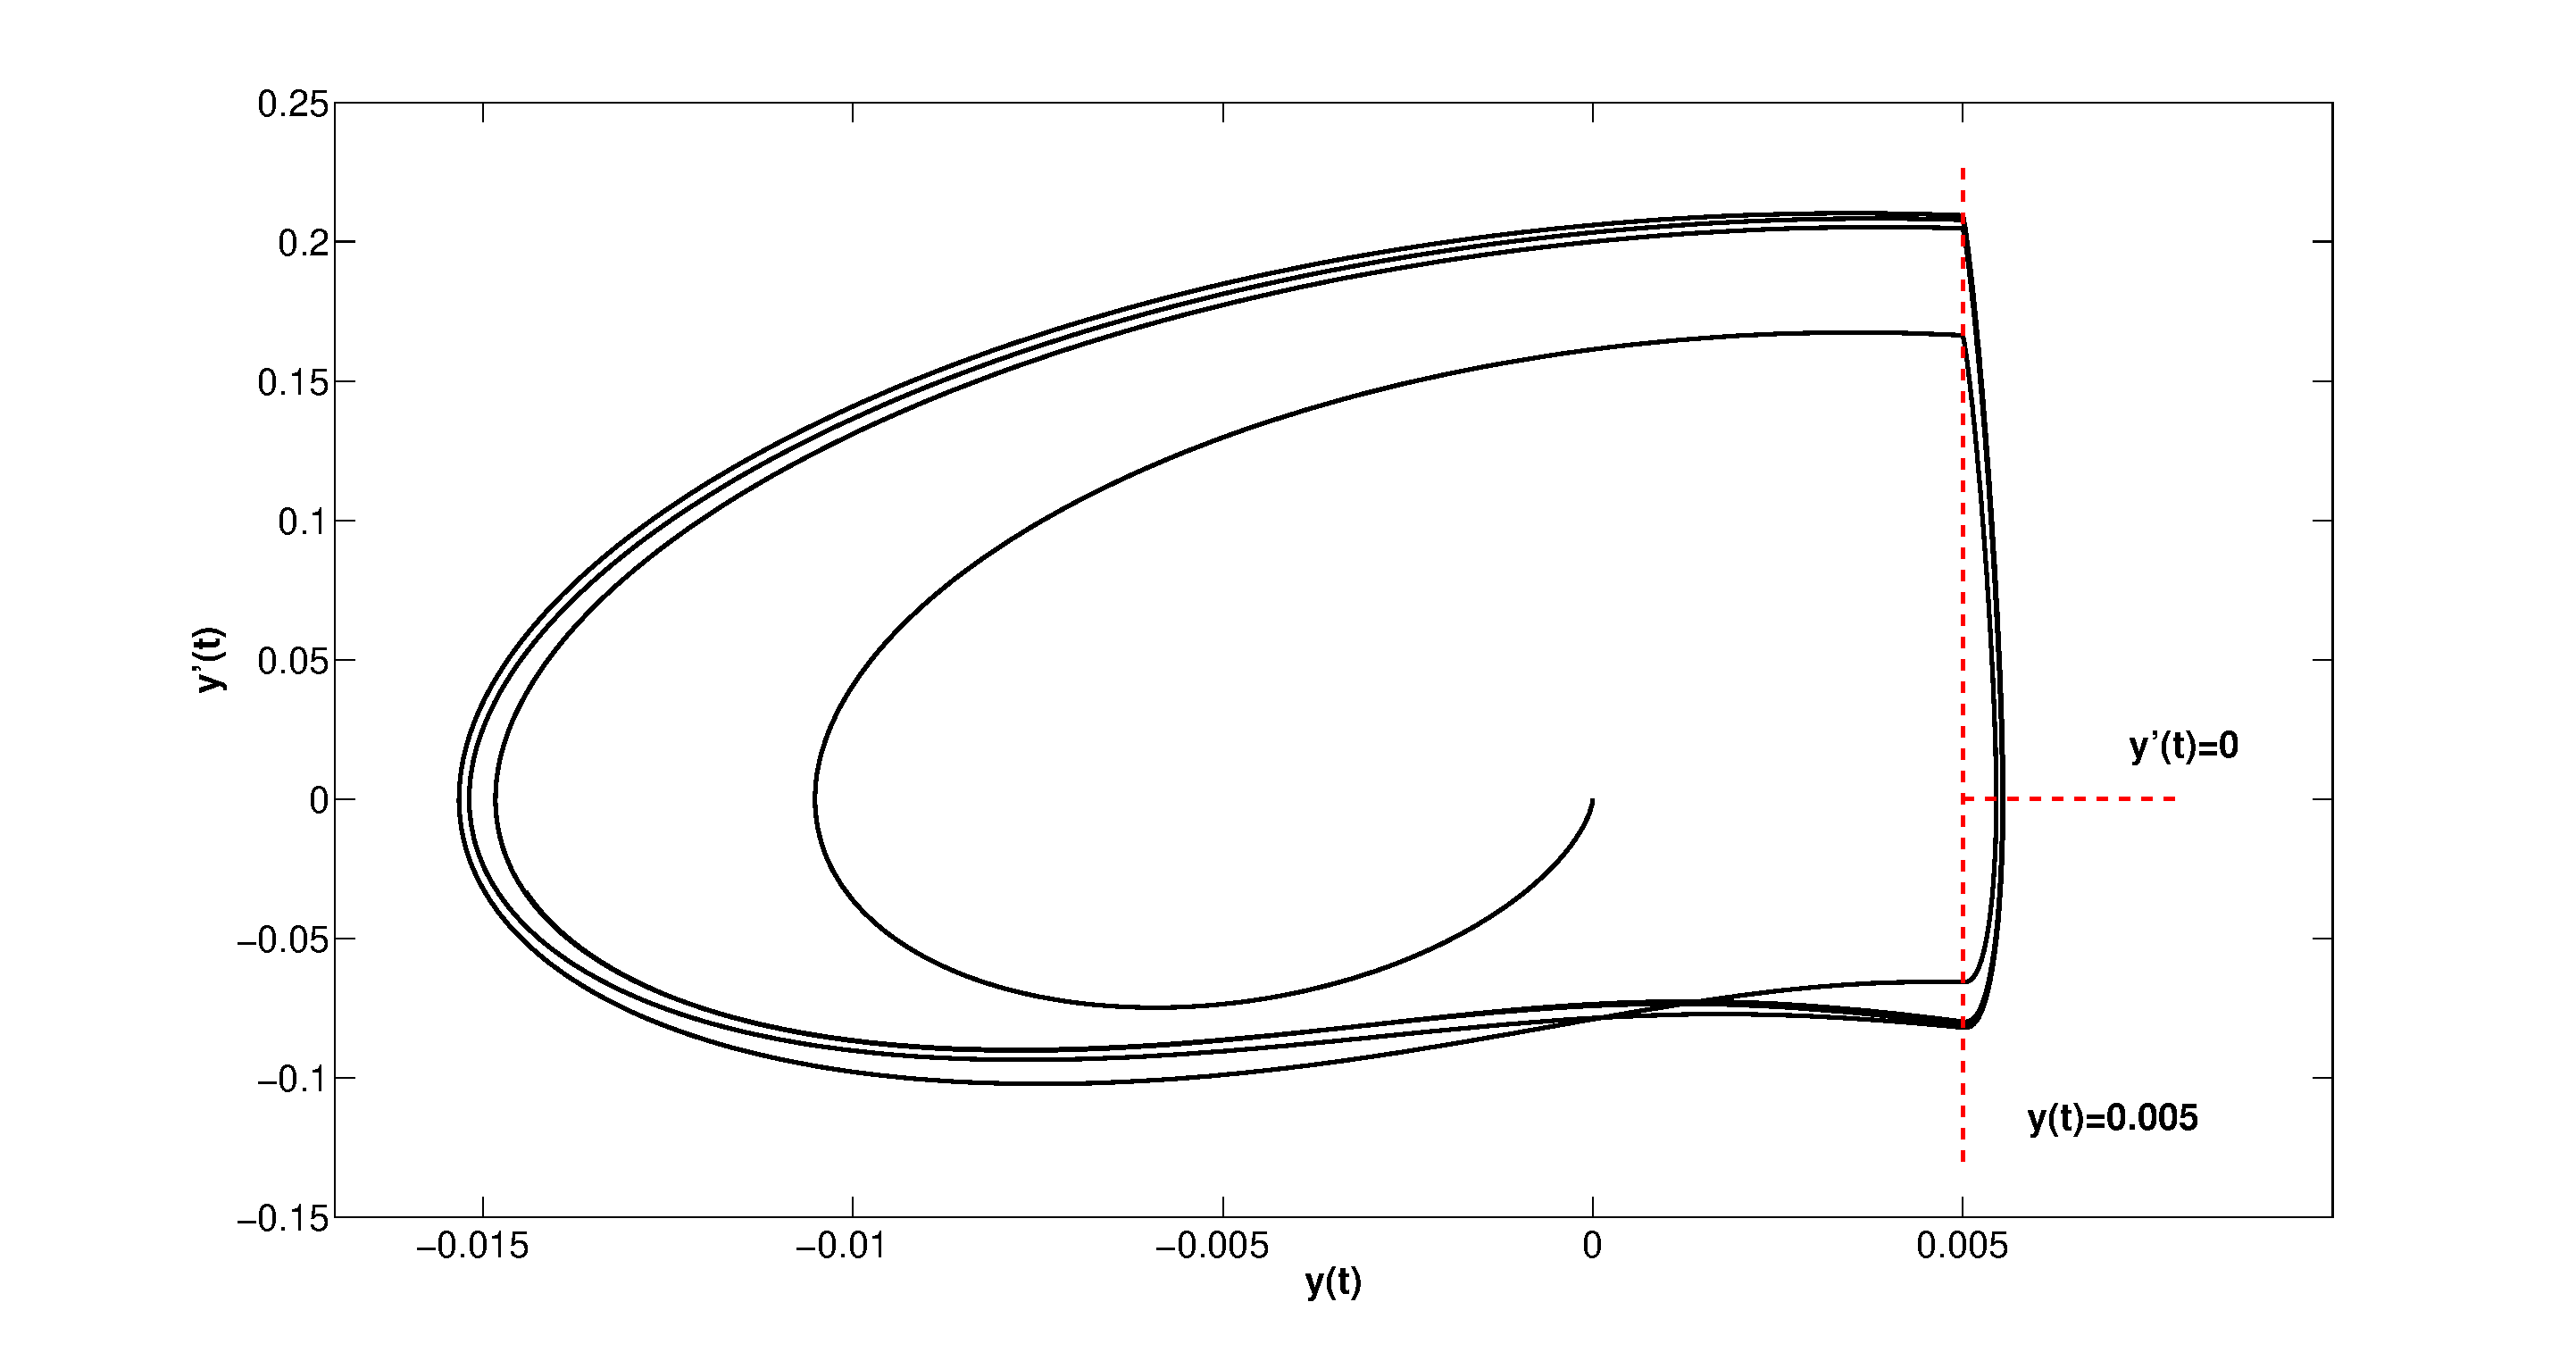
\includegraphics[width=15 true cm]{earthquake-phase}
}
\caption{Phase diagram for structural pounding model}
\label{Example4}
\end{figure}

The discontinuity points (where the third derivative $x'''(t)$ is not continuous)
lie onto the red dashed lines.


A Matlab code to integrate this problem with \texttt{disode45} can be

\bigskip

\begin{verbatim}
%
%  Call to disode45
%
 options=disodeset('Refine',10);
 y0 = [0;0];
 [tout,yout,tdis,ydis,idis,stats]=disode45(@fun4, ...
                                    @gfun4,[0,3], y0,options);
%
%  Definition of the vector field
%
 function f=fun(t,y)
      k=210.125;
      c=2.47e+6;
      nu=0.005;
      r=2*sin(14*t);
      if y(1)>nu
        if y(2)>0
           u=c*(y(1)-nu)^(3/2) + 1.98*sqrt(2*c*sqrt(y(1)-nu))*y(2);
        else
           u=c*(y(1)-nu)^(3/2);
        end
      else
        u=0;
      end
      f=[y(2); (-4.1*y(2)-k*y(1)-u-r)/2];
 end
%
%  Definition of the switching surfaces
%
 function [g,isterminal,direction]=gfun(t,y)
    if y(1)<0.005
       g=[y(1)-0.005;1];
    else
       g=[y(1)-0.005;y(2)];
    end
    isterminal=[0;0];
    direction=[0;-1];
 end
\end{verbatim}

Once the integration of this problem concludes, the vectors tdis, ydis
and idis contain the following data

\begin{verbatim}
tdis =

    0.4006    0.4071    0.4172    0.8384    0.8446    0.8543
    1.2818    1.2880    1.2977    1.7307    1.7368    1.7467
    2.1798    2.1860    2.1958    2.6286    2.6348    2.6446


  Columns 13 through 18

    2.1798    2.1860    2.1958    2.6286    2.6348    2.6446

ydis =

    0.0050    0.1664
    0.0055    0.0000
    0.0050   -0.0658
    0.0050    0.2095
    0.0055    0.0000
    0.0050   -0.0820
    0.0050    0.2079
    0.0055   -0.0000
    0.0050   -0.0811
    0.0050    0.2048
    0.0055    0.0000
    0.0050   -0.0799
    0.0050    0.2047
    0.0055    0.0000
    0.0050   -0.0799
    0.0050    0.2049
    0.0055    0.0000
    0.0050   -0.0799


idis =

      1     2     1     1     2     1     1     2     1
      1     2     1     1     2     1     1     2     1
\end{verbatim}

The plot in Figure \ref{Example4} (without legends) can be obtained with the matlab order

\begin{verbatim}
plot(yout(:,1),yout(:,2),[0.005,0.005],[-0.15,0.25],'r--', ...
                                    [0.005, 0.008],[0,0],'r--');
\end{verbatim}

\item[Example 5]
A bouncing ball model (ODE with impulses) is governed by the equation
\[
x''=-9.8.
\]
Starting from a height $x(0)=x_0$ with velocity $x'(0)= x'_0$, the ball falls  and when it
attains the floor $x(t_d)=0$, with velocity $x'(t_d)=x'_d$,
the integration must be restarted with initial conditions $x(t_d)=0$,
$x'(t_d)=-0.9\; x'_d$ where the factor $0.9$ represents the lost of energy.

Expressed as a first order system with
two components $y_1(t)=x(t)$, $y_2(t)=x'(t)$, we have
\[
y'=\begin{pmatrix} y_1' \\y'_2 \end{pmatrix}=
\begin{pmatrix} y_2 \\ -9.8
\end{pmatrix} = f(t,y)
\]

\medskip

Here the switching surface is clearly $g(y)=y_1$.

In this case the discontinuity affects the solution, and the jump of the
state must be provided in some way by the user.  In the code this is done by means
of an external function \texttt{actionatswitch(t,y)} that from the current state
$y_d$ provides the new state $y_d^*$.

A Matlab code to integrate this problem with \texttt{disode45} can be

\bigskip

\begin{verbatim}
%
 options=disodeset('AbsTol',1.e-4,'RelTol',1.e-4, ...
                 'Refine',10, 'ActionSwitch',@actionatswitch);
 y0=[10; 0];
 [tout,yout,tdis,ydis,idis,stats]=disode45(@fun, ...
                              @gfun,[0,20], y0, options);
%
%  Definition of the vector field
%
 function ydot=fun(t,y)
      ydot=[y(2); -9.8];
 end
%
 function [g,isterminal,direction]=gfun(t,y)
      g=y(1);
      isterminal=-1; %  Call to gwhenswitch when a switching point is found
      direction=-1;
 end
 %
 %  Output switch function
 %
 function ysw=actionatswitch(t,y)
       ysw=[0; -0.9*y(2)];
 end
 \end{verbatim}

Once the integration of this problem concludes, the vectors \texttt{tdis}, \texttt{ydis}
and \texttt{idis} contain the data corresponding to 13 switching points.

\begin{verbatim}
tdis =

     1.4286    4.0000    6.3143    8.3971   10.2717   11.9588   13.4772
    14.8438   16.0737   17.1806   18.1768   19.0734   19.8804

ydis =

    0.0000  -14.0000
   -0.0000  -12.6000
   -0.0000  -11.3400
   -0.0000  -10.2060
   -0.0000   -9.1854
    0.0000   -8.2669
    0.0000   -7.4402
    0.0000   -6.6962
   -0.0000   -6.0265
    0.0000   -5.4239
   -0.0000   -4.8815
   -0.0000   -4.3933
   -0.0000   -3.9540
\end{verbatim}

\item[Example 6]
A heating model (problems with a switching vector field).  The variation
of the temperature in a room is supposed to be linear on the difference
$x(t)- T_{\hbox{\scriptsize ext}}$
between the current temperature $x(t)$ and the external temperature
$T_{\hbox{\scriptsize ext}}$.
Initially, if the temperature
$x(0)$ is lower than a maximum temperature $T_{\max}$, the heating is on,
a constant external heat source $u$ is acting and the temperature
satisfies the equation
\[
x'=-K\cdot (y-T_{\hbox{\scriptsize ext}})+u,
\]
until the temperature attains $T_{\max}$.  At that moment the heat source $u$
is set off and the differential equation changes to
\[
x'=-K\cdot (y-T_{\hbox{\scriptsize ext}}).
\]
The heat source is set on again when $x(t)= T_{\min}$.

Note that in this example
the vector field itself is modified from $f(t,x)$ to a different one
$\hat f(t,x)$ when the solution
attains certain point $t_d$ satisfying a condition $g(t_d,x(t_d))=0$.
For the same point $(t,x)$, the vector field
$f(t,x)$ can not be equal to  $\hat f(t,x)$.

In order to solve this problem with DISODE45, it must be transformed, by adding an additional equation, into an equivalent problem that can be treated as an ODE with impulses.  Defining
$y(t)=(y_1(t), y_2(t))^T \equiv (x(t), y_2(t))^T$, where $y_2(t)$ is going to be a constant,
the heating can be modelled by
\[
\begin{array}{l}
y_1'=\begin{cases}
-K\cdot(y_1-T_{\hbox{\scriptsize ext}})+ u & \hbox{if } y_2(t) =1, \\
-K\cdot(y_1-T_{\hbox{\scriptsize ext}})& \hbox{if } y_2(t) =-1,
\end{cases}
\\
y_2'= 0, \\
y_1(0)=x(0)= x_0, \quad y_2(0)=
\begin{cases}
1 & \hbox{ if }  x_0 < T_{\max},\\
-1 &  \hbox{ if }  x_0 \ge  T_{\max}. \end{cases}
\end{array}
\]
There are two switching surfaces $g_1(y)=y_1-T_{\max}$ and
$g_1(y)=y_1-T_{\min}$.  When the solution attains the first one from temperature
$x(t) <T_{\max}$, or the second one from temperature $x(t) > T_{\min}$,
the sign of the variable $y_2(t_d)$ is changed.

A Matlab code to integrate this problem with \texttt{disode45} can be

\bigskip

\begin{verbatim}
%
 options=disodeset('AbsTol',1.e-4,'RelTol',1.e-4,'ActionSwitch',@actionatswitch);
 y0=[15;1];
 [tout,yout,tdis,ydis,idis,stats]=disode45(@fun, @gfun,[0,20], y0, options);
%
 function ydot=fun(t,y)
     if y(2)==-1
       ydot=[-0.1*(y(1)-18); 0] ;
     else
       ydot=[-0.1*(y(1)-18)+2; 0] ;
     end
 end
%
 function [g,isterminal,direction]=gfun(t,y)
      g=[y(1)-23.5; y(1)-22];
      isterminal=[-1;-1];  %  Call to actionatswitch when found
      direction=[1;-1]; % From negative to positive the first one
 end
 %
 %  Output switch function
 %
 function yswitch=actionatswitch(t,y)
     if y(2)==1,
       yswitch=[y(1); -1];
     else
       yswitch=[y(1); 1];
     end
 end
 \end{verbatim}

 Once the integration of this problem concludes, the vectors \texttt{tdis}, \texttt{ydis}
and \texttt{idis} contain the data corresponding to 13 switching points.

\begin{verbatim}
tdis =

    4.6135    7.7980    8.7824   11.9669   12.9513   16.1359   17.1203

ydis =

   23.5000    1.0000
   22.0000   -1.0000
   23.5000    1.0000
   22.0000   -1.0000
   23.5000    1.0000
   22.0000   -1.0000
   23.5000    1.0000

idis =

     1     2     1     2     1     2     1
\end{verbatim}
\end{description}

\bigskip

\baselineskip=0.9\normalbaselineskip

{\small
\begin{thebibliography}{99}

\bibitem{AcaBro:08} V. Acary and B. Brogliato,
{\sl Numerical Methods for Nonsmooth Dynamical Systems} (Lecture Notes in Applied and Computational Mechanics, Springer--Verlag, Berlin,
2008).

\bibitem{CaMoRa:05} M. Calvo, J.I. Montijano  and  L. R\'{a}ndez,
{\em DISODE45, A Matlab Runge-Kutta solver for Piecewise
Smooth IVPs of Filippov type}, to appear in ACM TOMS.

\bibitem{Jank:05}
{\rm  R. Jankovski}, {\em Non-linear viscoelastic modelling of earthquake-induced
structural pounding},
Earthq. Eng. Struct. Dyn. 34(2005), pp.~595-611.

\bibitem{Luo} A.C.J. Luo,
{\sl Discontinuous Dynamical Systems on Time-varying Domains}
(Nonlinear Physical Science, Springer--Verlag, Berlin, 2009
).
\end{thebibliography}
\end{document}
